%-------------------------------------------------------------------------------
% Preamble
%-------------------------------------------------------------------------------

\documentclass[a4paper, 12pt]{article}
\usepackage[margin=2cm]{geometry}
\usepackage[osf]{mathpazo} % palatino
%\usepackage[round]{natbib} % author-year citations
\usepackage[superscript,biblabel]{cite} % for superscript citations
\usepackage{graphicx}
\usepackage{subcaption}
\usepackage{parskip} 
\usepackage{amsmath}
\usepackage{longtable}
\usepackage{pdflscape}
\usepackage{array}
\usepackage{float}
\usepackage{url}

\pagenumbering{arabic}  
\linespread{1.3}

% figure numbering override
\renewcommand*{\thefigure}{A\arabic{figure}} % make Fig A1 not Fig 1
\renewcommand*{\thetable}{A\arabic{table}} % make Table A1 not Table 1

%-------------------------------------------------------------------------------
% Title page information
%-------------------------------------------------------------------------------

\title{Supplementary Materials from: \textit{TITLE}; journal}

\author{Tara Wainwright, 
  Morwenna Trevenna, 
  Sarah Alewinjse,\\ 
  Marc E.H. Jones, 
  Jeff? 
  Patrick? and\\
  Natalie Cooper}

\date{}

% End of preamble

\begin{document}

\maketitle

\tableofcontents

\parindent = 1.5em
\addtolength{\parskip}{.3em}

%-------------------------------------------------------------------------------
% Supplementary materials
%-------------------------------------------------------------------------------
\newpage
\section{Numbers of specimens for each species}
%-------------------------------------------------------------------------------
We expect large skews in the proportion of male or female specimens when sample size is low, but the ratio of male:female specimens should approach 50:50 as more specimens are added if there is no bias. 
Most species in our dataset were represented by only a few specimens (Figure \ref{fig-histograms}; median of 8 specimens for each species), with large skews in the percentage of female specimens (in both directions) at low numbers (Figure \ref{fig-hex}).
To test whether this may influence our analyses, we used generalised linear models (GLM) with binomial errors, with the proportion of female specimens (success) and the proportion of male specimens (failure) for each species as the response variable, and the log number of specimens per species as the explanatory variable. 
We then used standard model checks for GLMs (Q-Q plot, histogram of residuals, residuals vs. linear predictors, response vs. fitted values) to assess model fit. 
The model showed massive heteroscedasticity in the residuals, due to the skew in proportions when sample size is low. 
We therefore repeated the analysis, removing species with fewer than 10, 25, 50 and 100 specimens in turn. 
The best fitting model, without losing too much data, was a model with species with more than 10 specimens. 
There is no significant relationship between the number of specimens and the proportion of female specimens using a minimum of 10 specimens for each species (binomial GLM: $deviance = 0.741$, $df = 1,3306$, $p = 0.389$) so we exclude this variable from further analyses.

% figure A1
\begin{figure}[H]
 \centering
  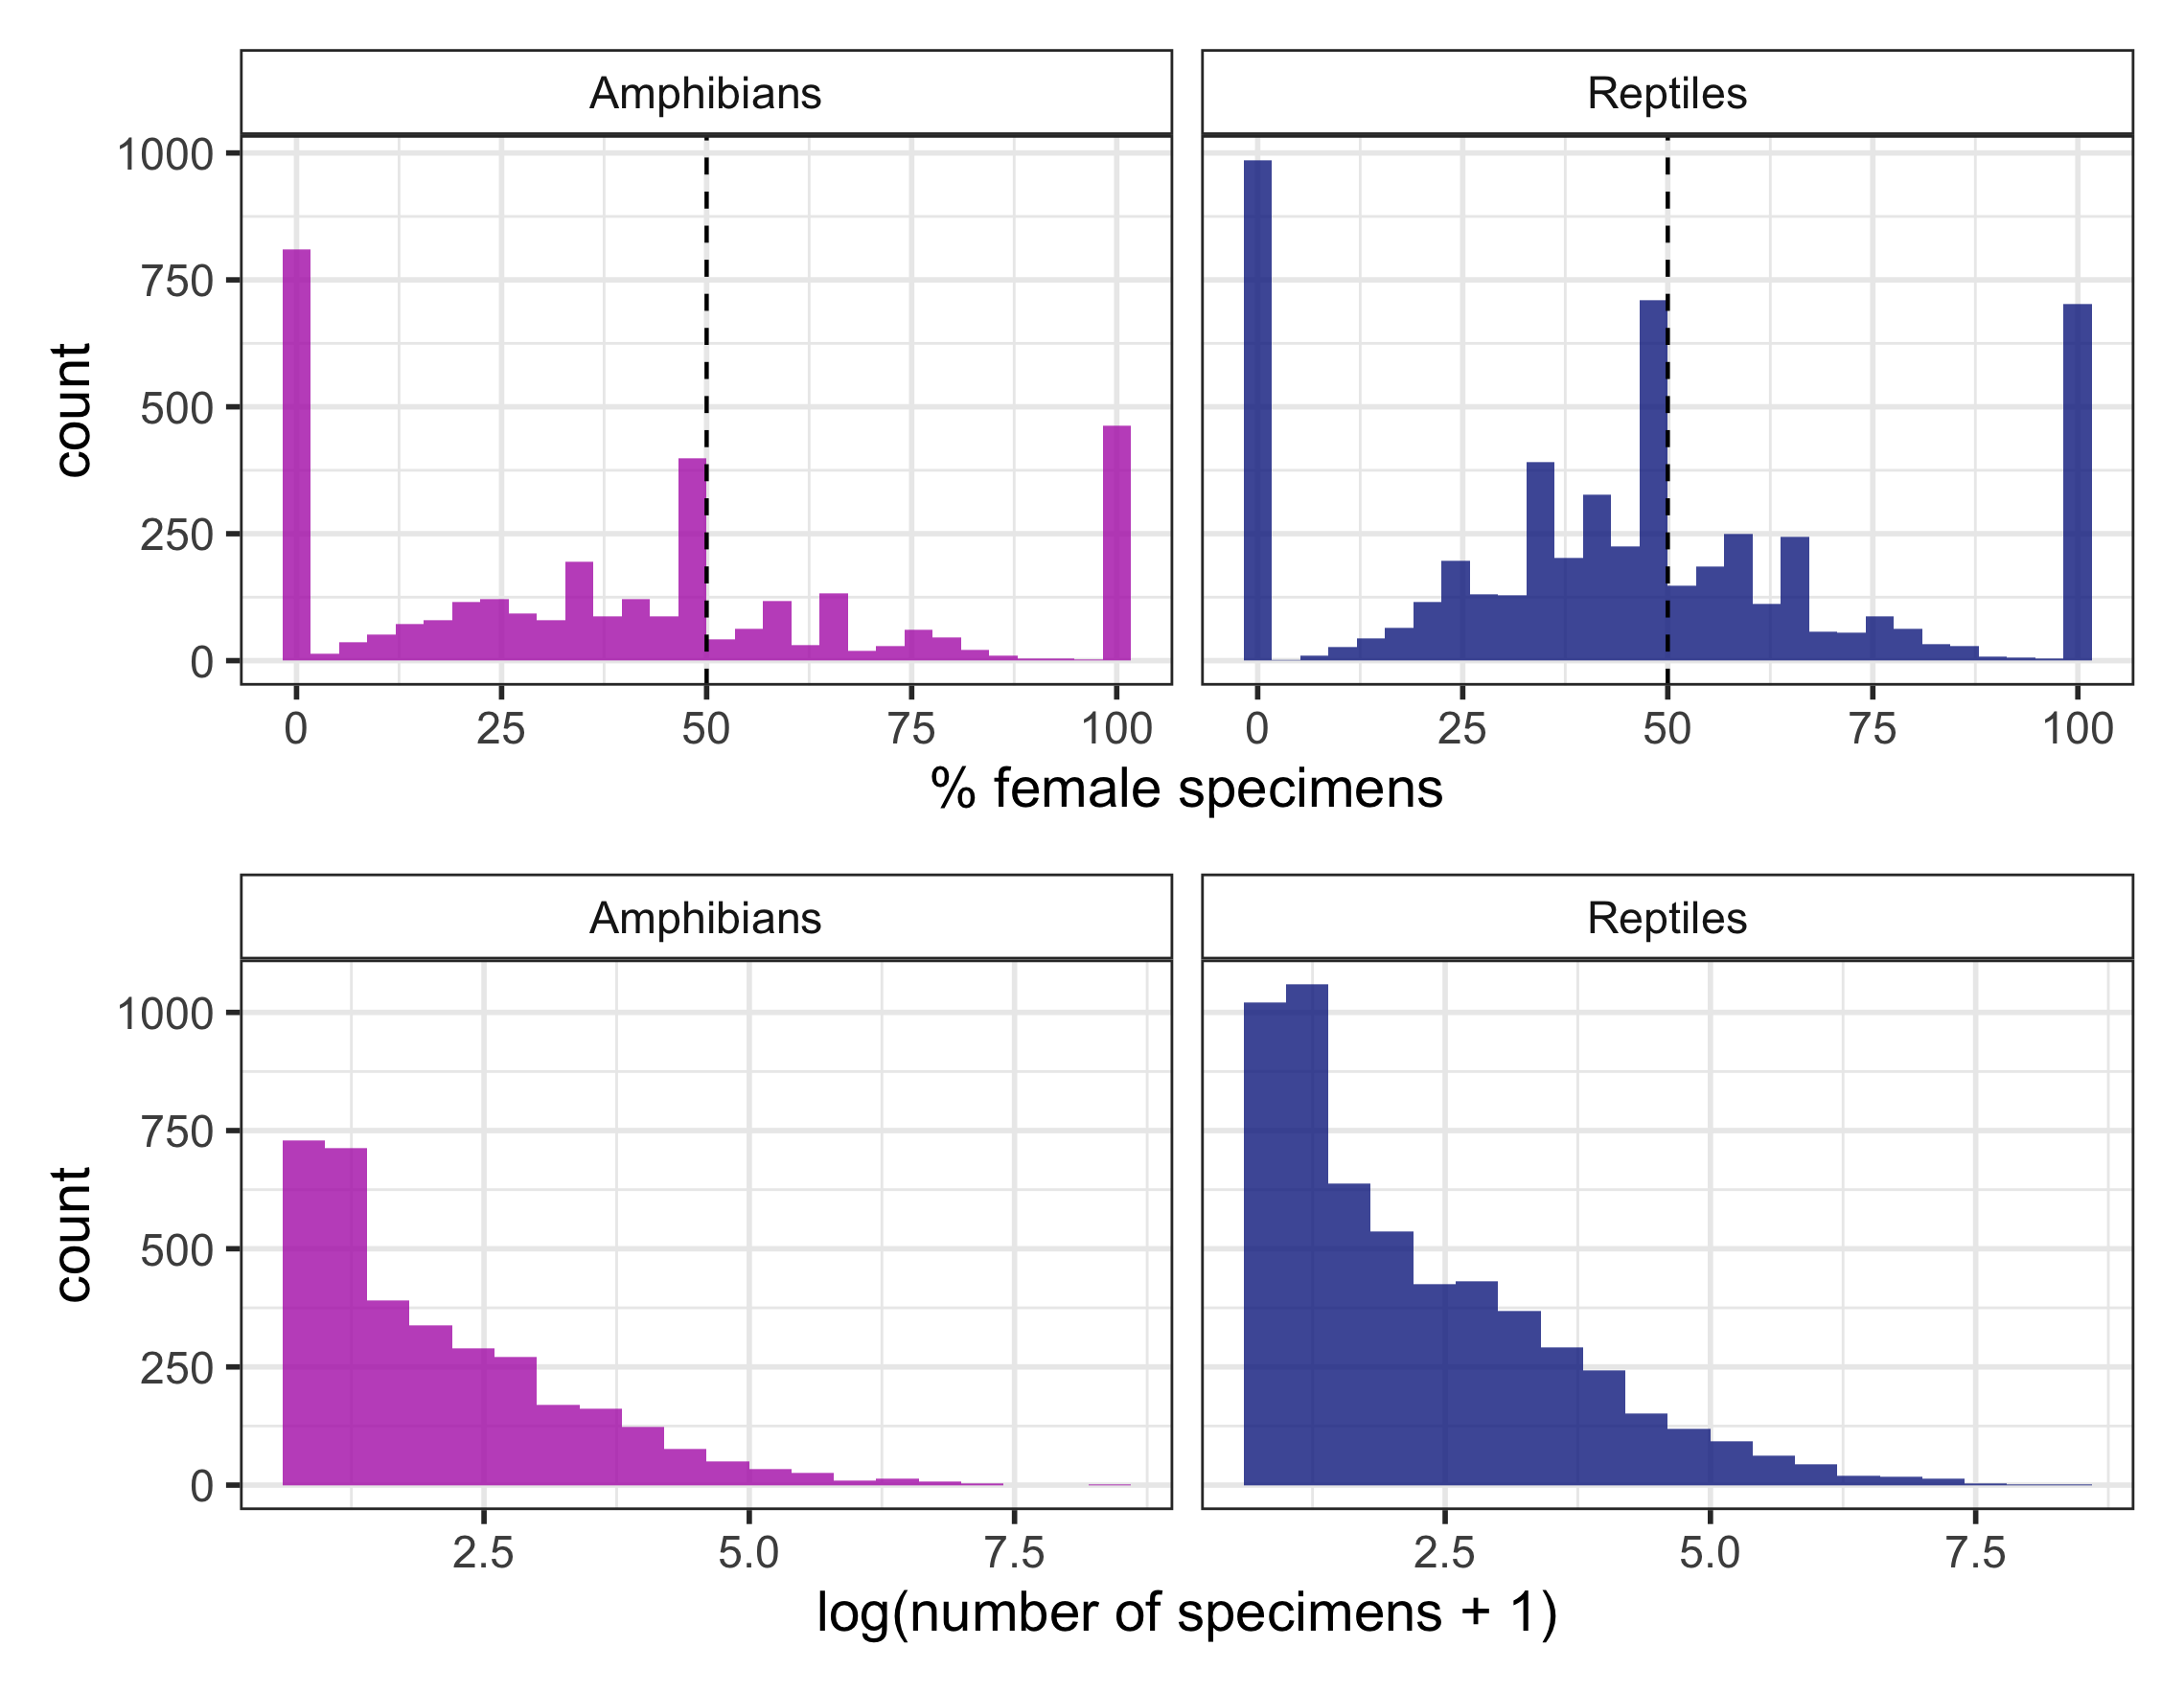
\includegraphics[width = \linewidth]{figures/histogram-specimen-counts.png}
  \caption{Histograms showing the distribution of percentage female specimens and log number of specimens for each species across amphibians and reptiles.}
  \label{fig-histograms}
\end{figure}

% figure A2
\begin{figure}[H]
 \centering
  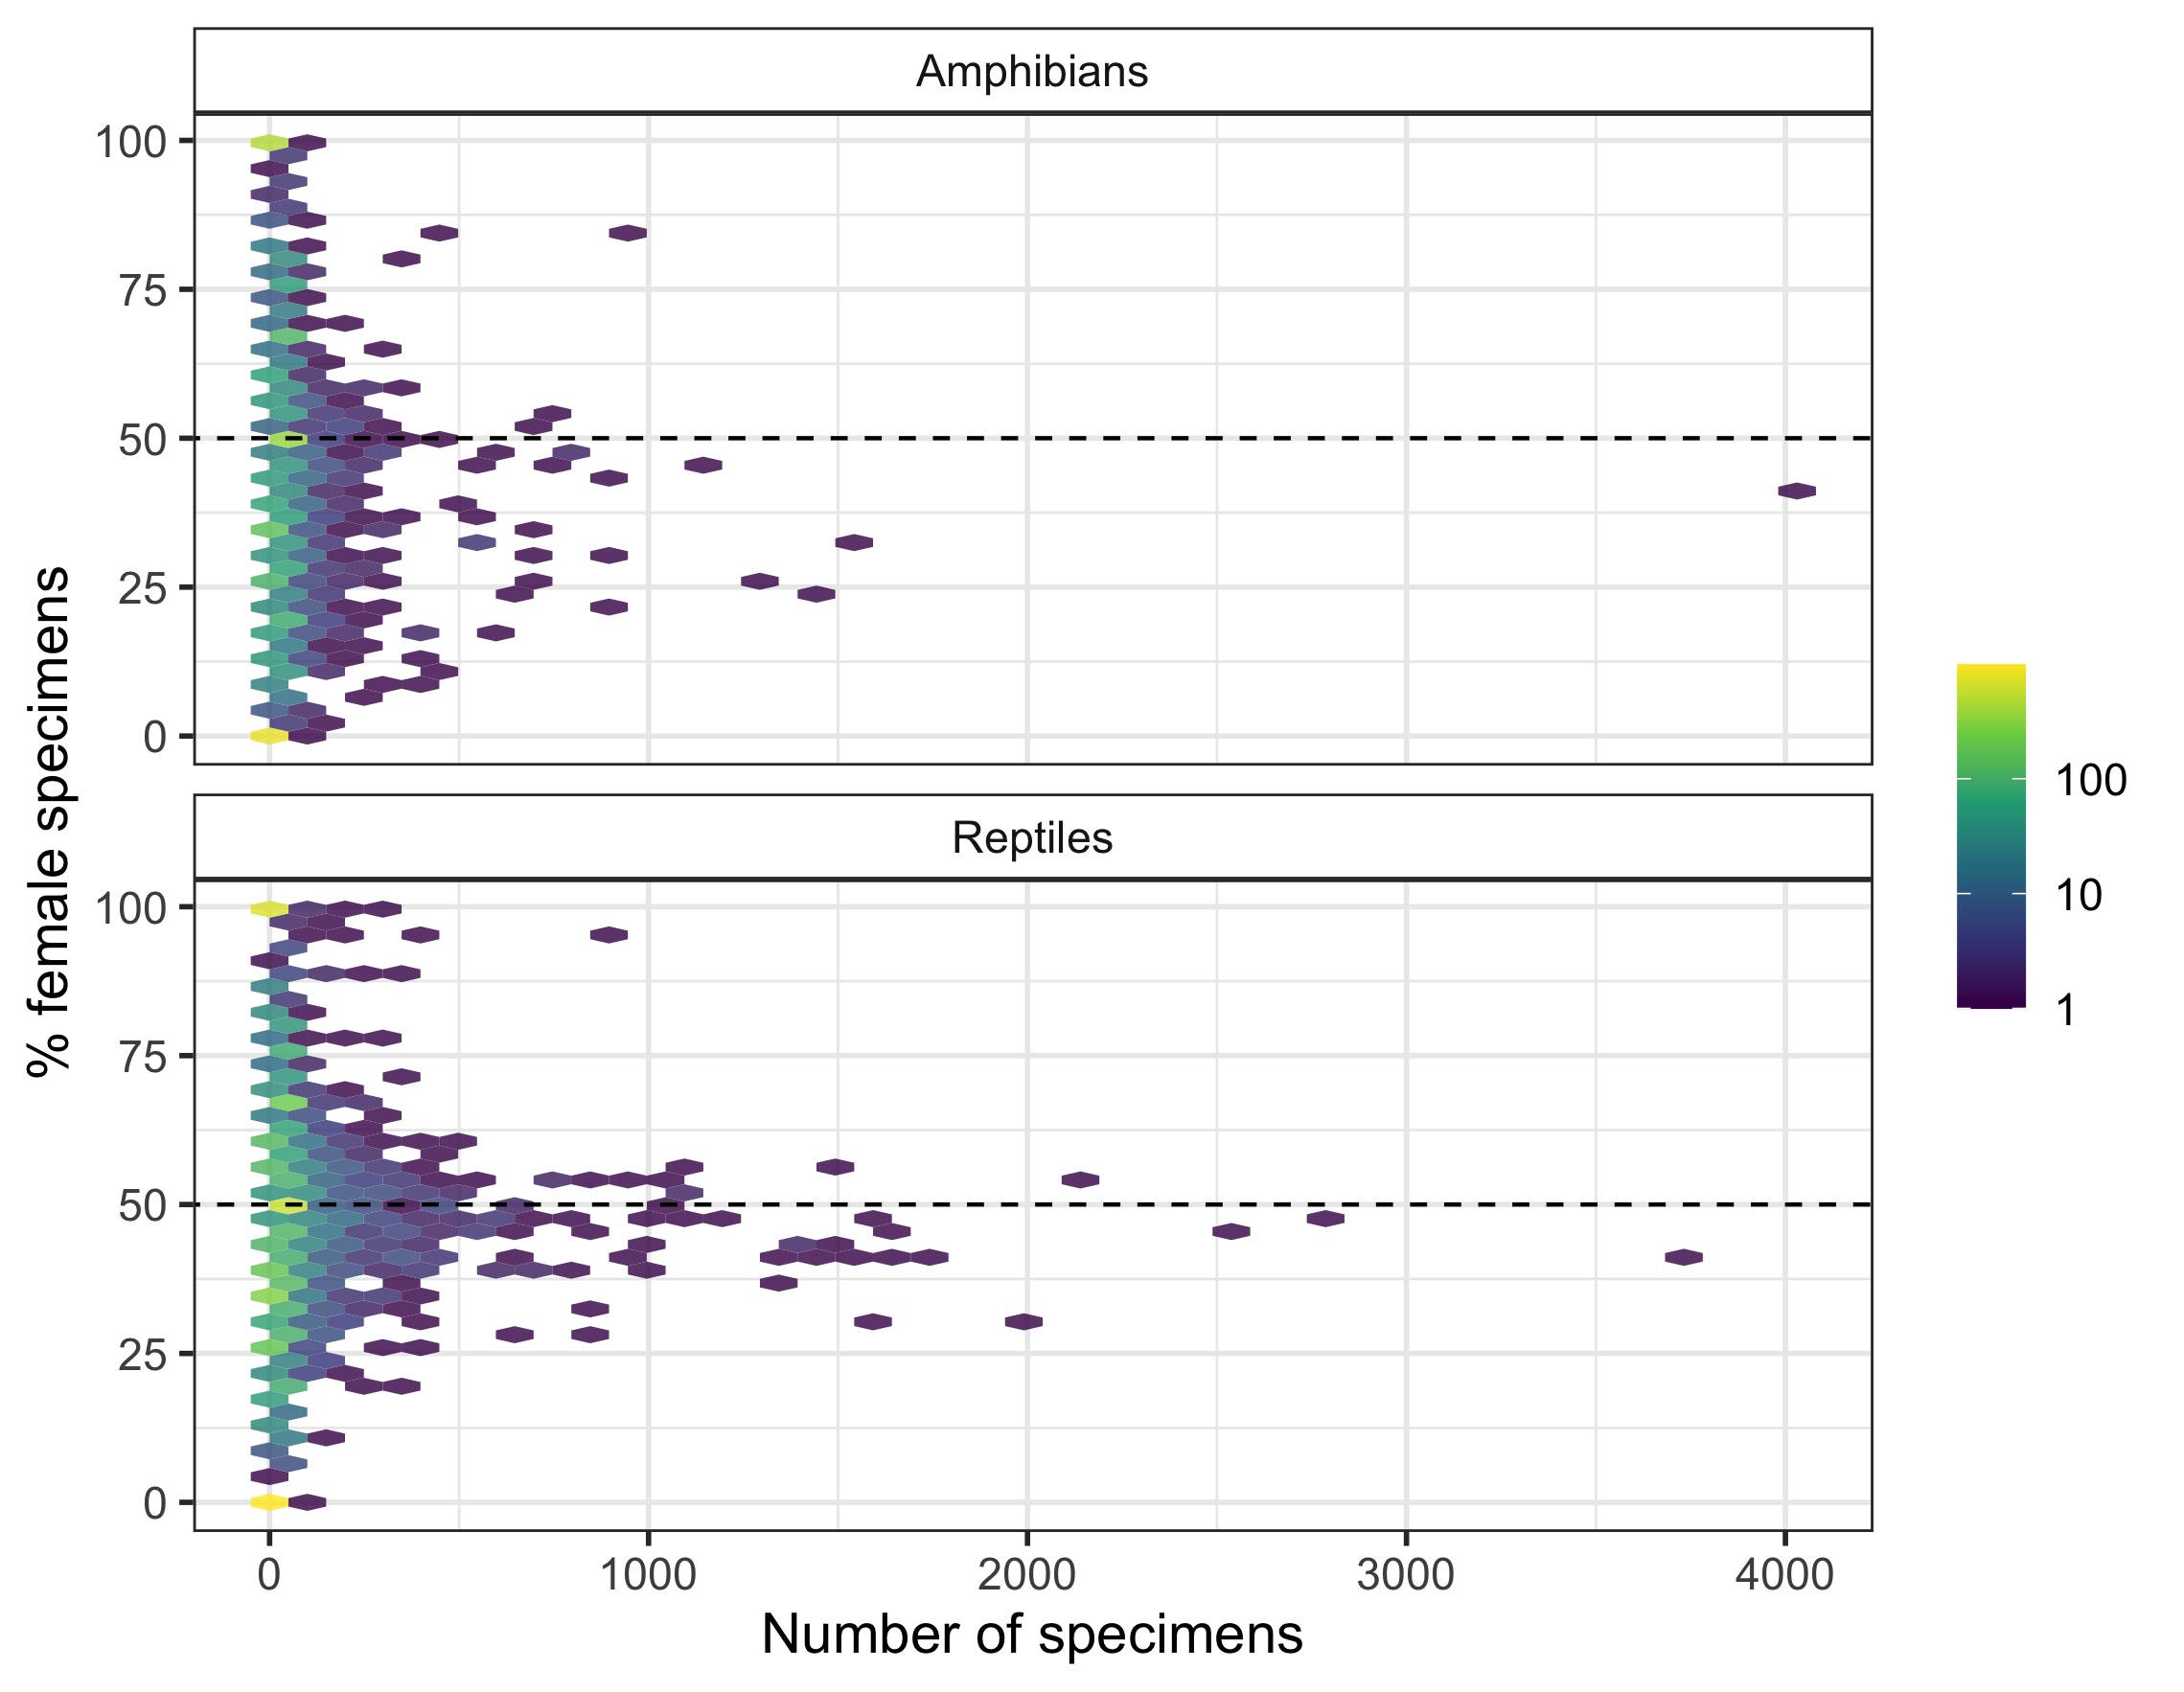
\includegraphics[width = \linewidth]{figures/specimens-numbers-all.png}
  \caption{Relationship between the percentage female specimens in each species and the number of specimens for each species across amphibians and reptiles. 
  Hex bins are used rather than points to make the plot easier to read.}
  \label{fig-hex}
\end{figure}

%------------------------------------------------------------------------------------------------
\newpage
\section{Total numbers of female, male, sexed and unsexed specimen and name-bearing type records}
%-------------------------------------------------------------------------------------------------
% Table A1
% Table A1
% Numbers from 01-summary-stats

\begin{longtable}{ccccc}

\caption{Numbers of specimens in our dataset divided by sex.}\\ 
  
\hline
\multicolumn{2}{c}{\textbf{AMBHIBIANS}} & \multicolumn{2}{c}{\textbf{REPTILES}} \\
\hline
% From kable sum1
  \multicolumn{5}{c}{\textbf{All specimens}}\\  
  \hline
  & \textbf{N specimens} & \textbf{\%} & \textbf{N specimens} & \textbf{\%}\\
  \hline
  Total & 2,753,451 & NA & 3,183,804 & NA\\
  Sexed & 82,577 & 3.00 & 194,496 & 6.11\\
  Unsexed & 2,670,874 & 97.00 & 2,989,308 & 93.89\\
  Female & 31,905 & 1.16 & 90,296 & 2.84\\
  Male & 50,672 & 1.84 & 104,200 & 3.27\\
  \hline

%from kable sum2
  \multicolumn{5}{c}{\textbf{Sexed specimens only}}\\
  \hline
  & \textbf{N specimens} & \textbf{\%} & \textbf{N specimens} & \textbf{\%}\\
  \hline
  Total & 82,577 & NA & 194,496 & NA \\
  Female & 31,905 & 38.64 & 90,296 & 46.43\\
  Male & 50,672 & 61.36 & 104,200 & 53.57\\
  \hline

  \multicolumn{5}{c}{\textbf{Sexed specimens from species with $\geq$ 10 specimens}}\\
  \hline
  & \textbf{N specimens} & \textbf{\%} & \textbf{N specimens} & \textbf{\%}\\
  \hline
  Total & 75,248 & NA & 183,285 & NA\\
  Female & 28,971 & 38.50 & 85,300 & 46.54\\
  Male & 46,277 & 61.50 & 97,985 & 53.46\\
  \hline

\label{table_A1}
\end{longtable}







\newpage

% figure A3
\begin{figure}[H]
 \centering
  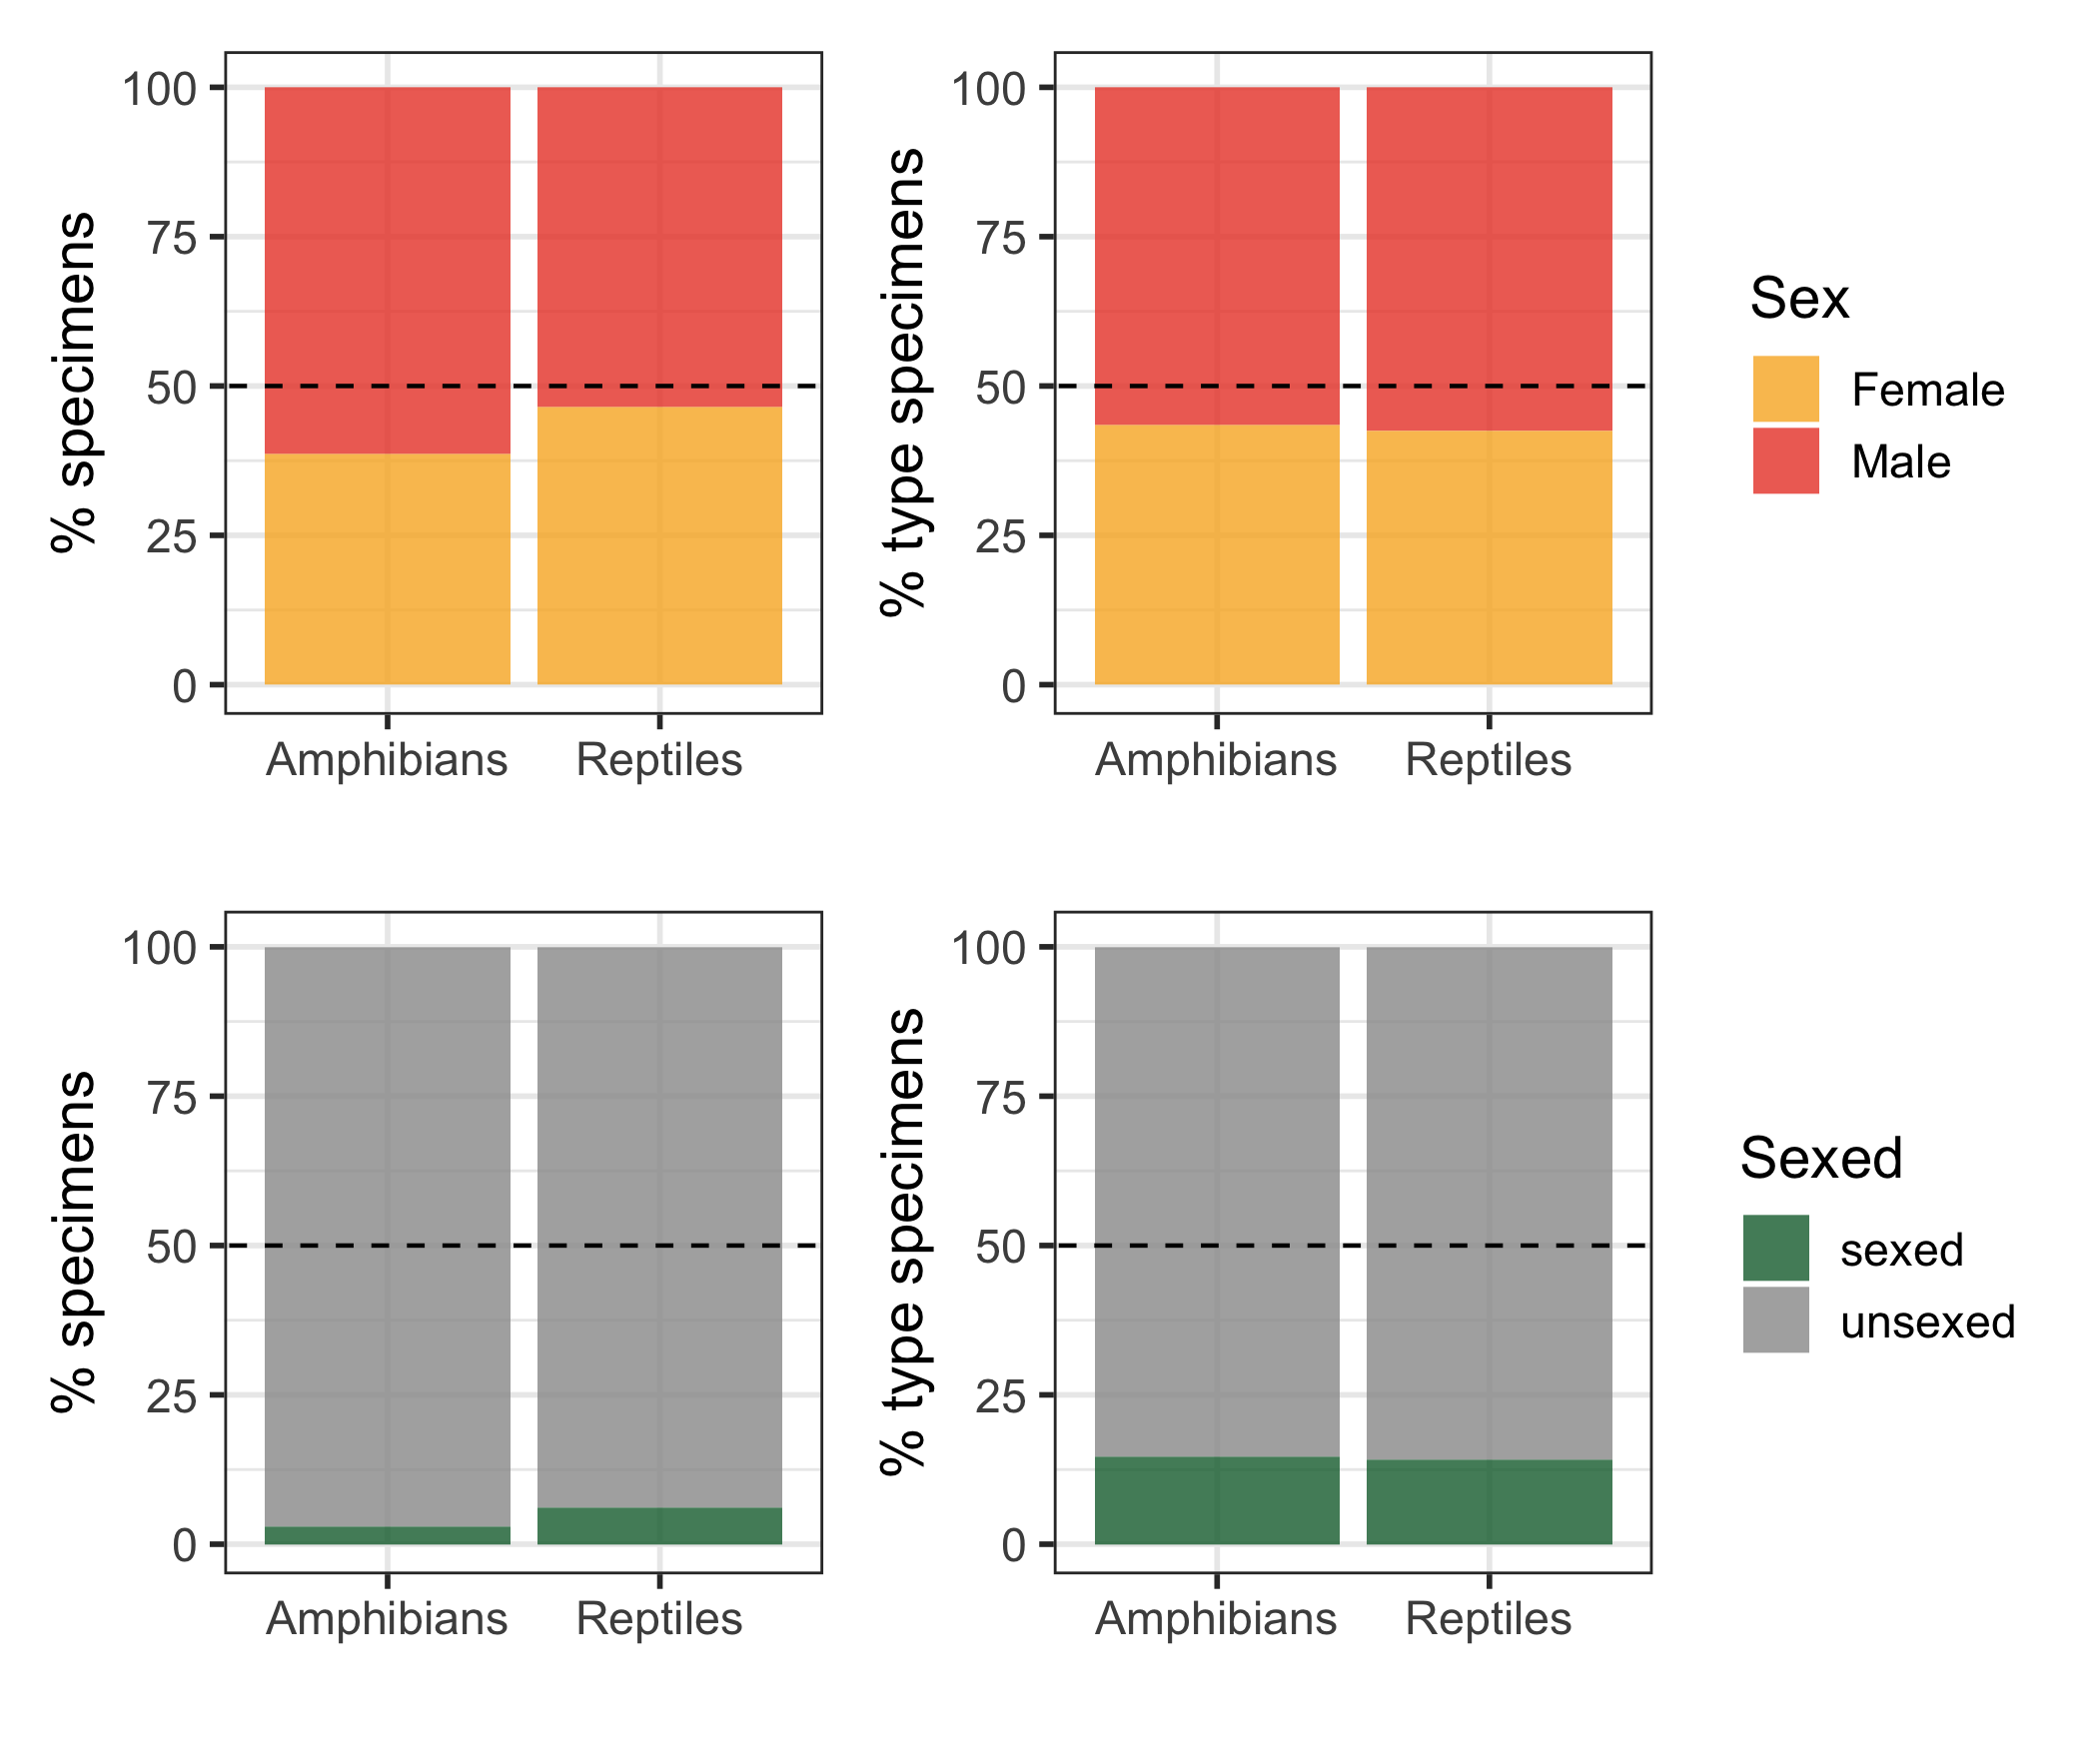
\includegraphics[width = \linewidth]{figures/types-class.png}
  \caption{Percentages of female (yellow), male (orange), sexed (green) and unsexed (grey) specimen records in amphibian and reptile collections for all specimens (left hand panels) and for name-bearing type specimens only (right hand panels). 
  The dashed line represents 50\% female specimens.}
  \label{fig-types-class}
\end{figure}

%------------------------------------------------------------------------------------------------
\newpage
\subsection{Orders}
%-------------------------------------------------------------------------------------------------

% figure A4
\begin{figure}[H]
 \centering
  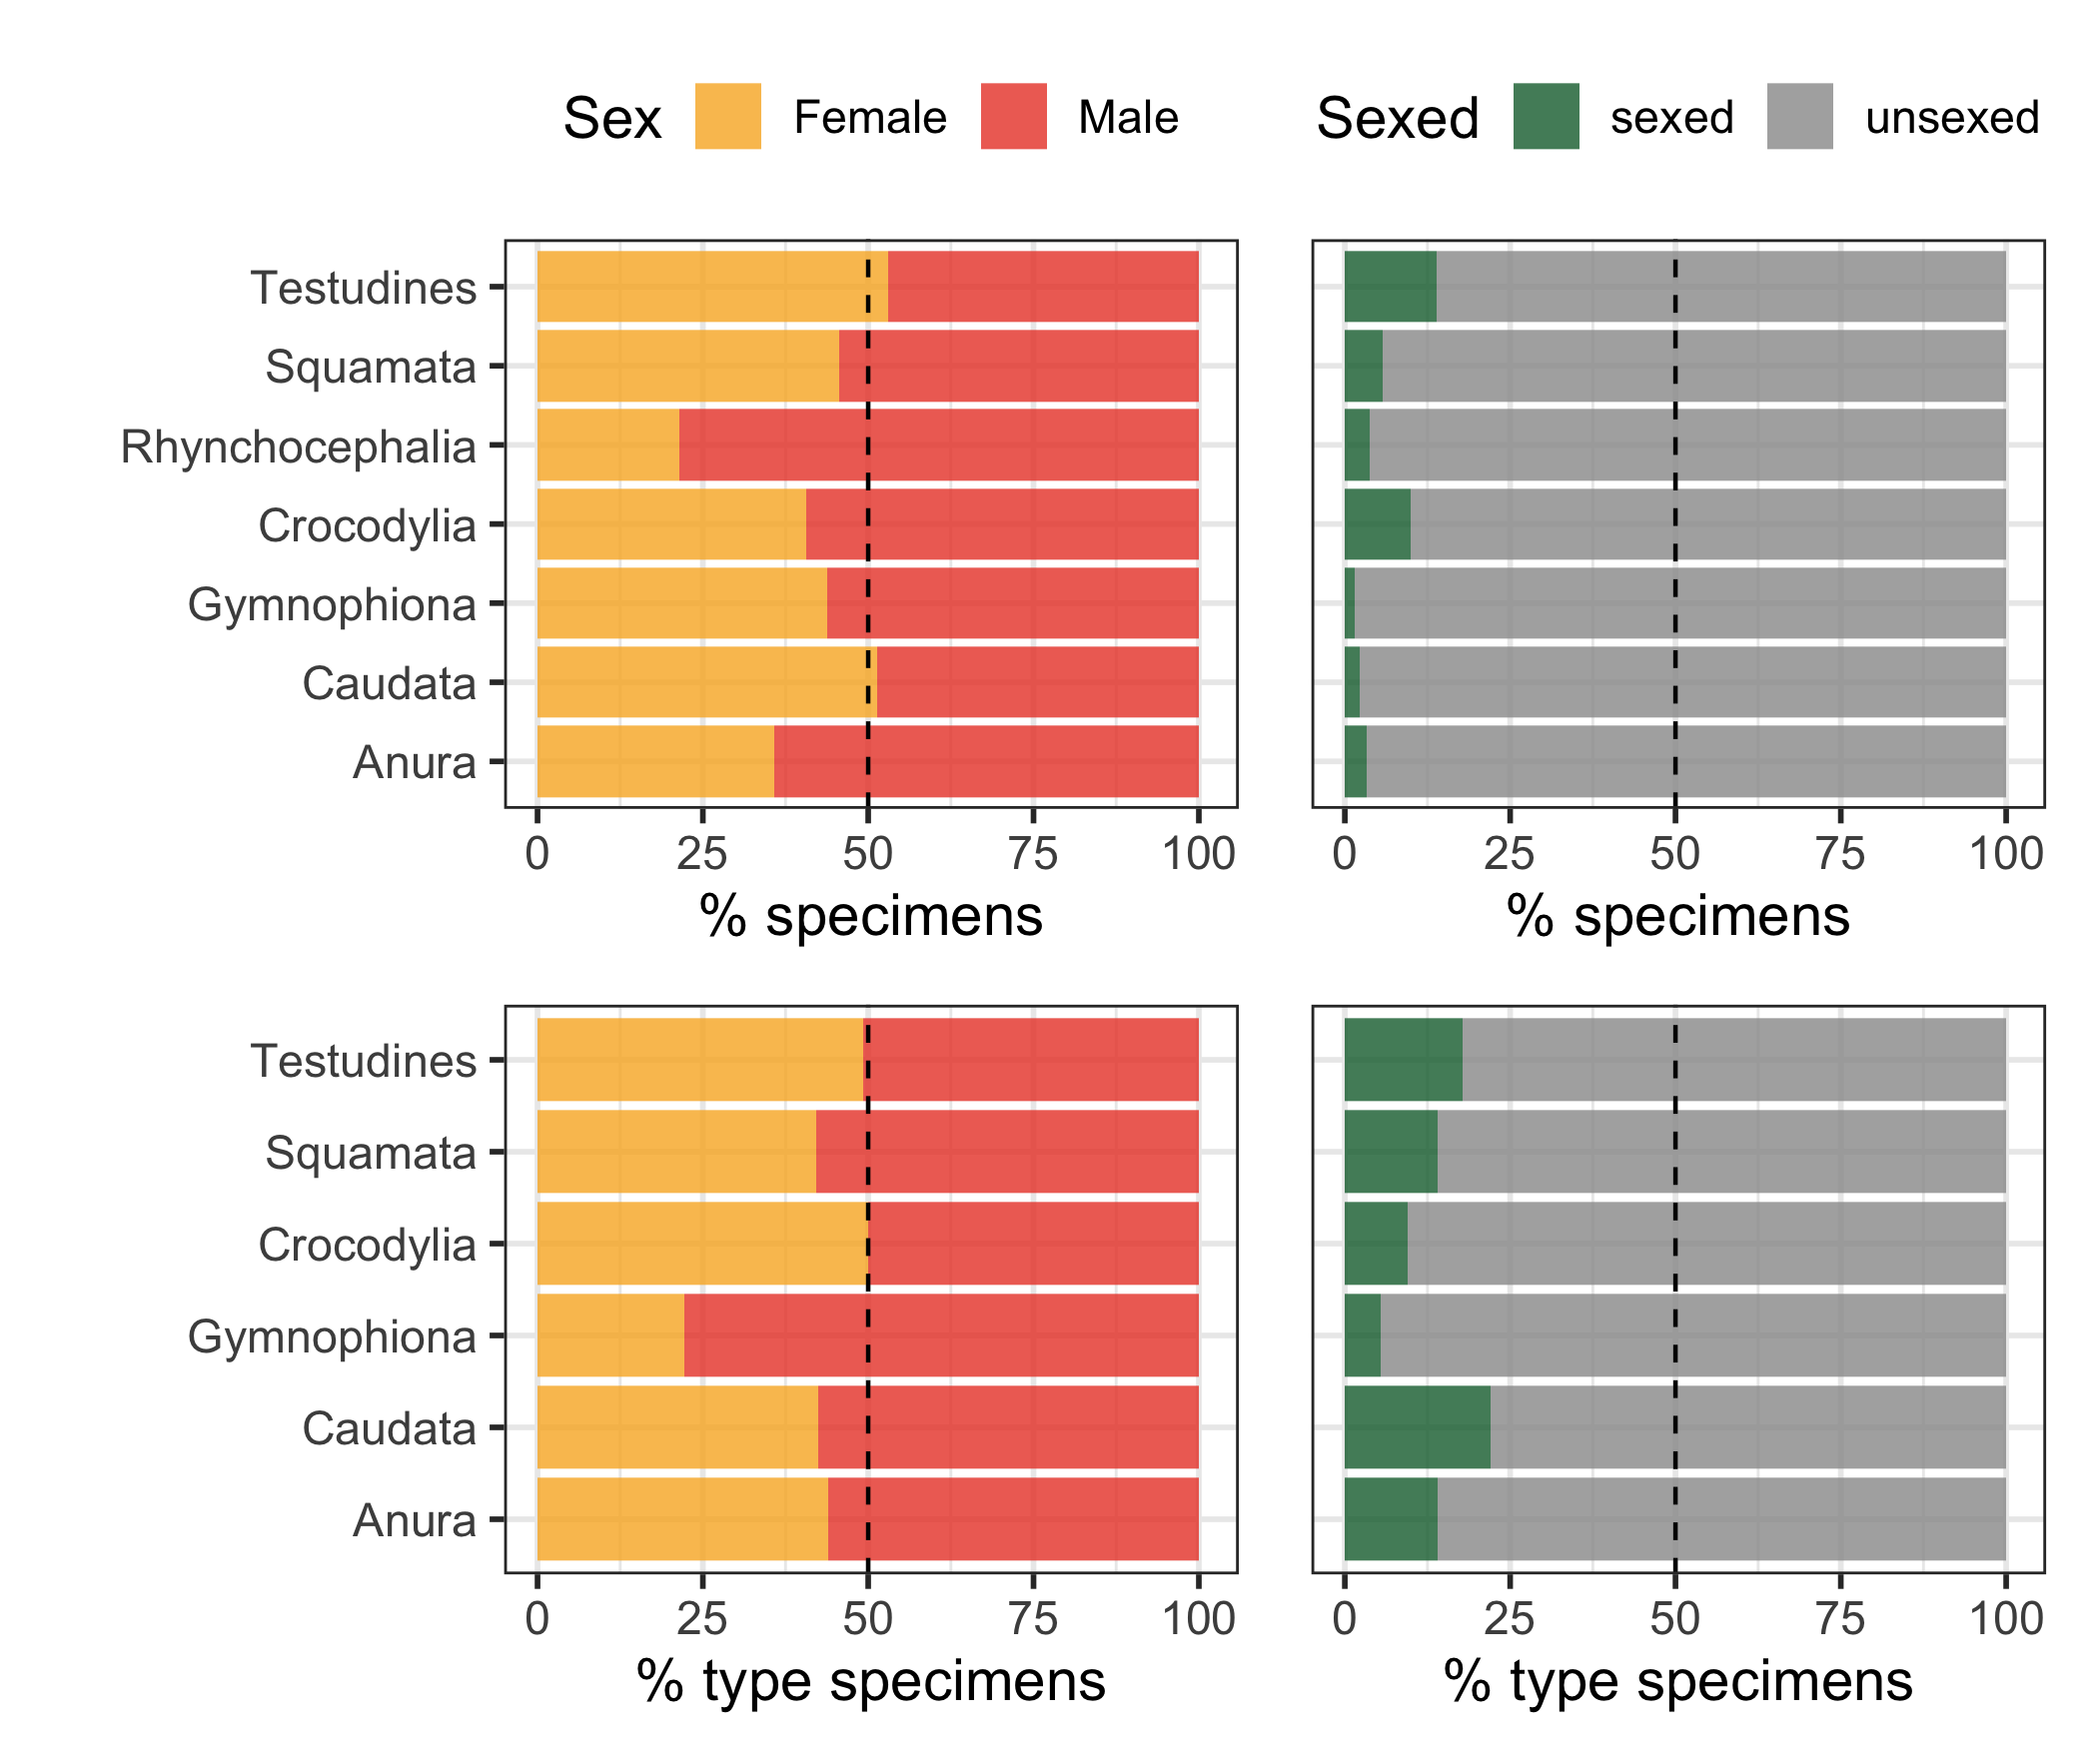
\includegraphics[width = \linewidth]{figures/types-order.png}
  \caption{Percentages of female (yellow), male (orange), sexed (green) and unsexed (grey) specimen records in amphibian and reptile collections for all specimens (top panels) and for name-bearing type specimens only (bottom panels), categorised by order. Rhynchocephalia is excluded from the name-bearing types plots as our dataset contained no types for this order. 
  The dashed line represents 50\% female specimens.}
  \label{fig-types-order}
\end{figure}

%------------------------------------------------------------------------------------------------
\newpage
\subsection{Families}
%-------------------------------------------------------------------------------------------------

\subsubsection{Amphibians}

% Table A2
% latex table generated in R 4.2.0 by xtable 1.8-4 package
% Tue Jul 26 14:17:47 2022
\begin{longtable}{llccc}
\caption{Percentages of female specimens for each family of amphibians.} \\ 
  \hline
order & family & n species & n specimens & \% female \\ 
  \hline
Anura & Allophrynidae &   1 &  18 & 50.00 \\ 
  Anura & Alsodidae &   9 & 915 & 63.93 \\ 
  Anura & Alytidae &   5 & 1000 & 50.00 \\ 
  Anura & Aromobatidae &  17 & 5430 & 61.33 \\ 
  Anura & Arthroleptidae & 101 & 180442 & 59.15 \\ 
  Anura & Ascaphidae &   2 & 868 & 50.00 \\ 
  Anura & Batrachylidae &   6 & 700 & 55.71 \\ 
  Anura & Bombinatoridae &   6 & 4422 & 56.22 \\ 
  Anura & Brachycephalidae &  25 & 3399 & 77.67 \\ 
  Anura & Brevicipitidae &  14 & 2024 & 70.45 \\ 
  Anura & Bufonidae & 293 & 5345748 & 63.57 \\ 
  Anura & Calyptocephalellidae &   1 &   4 & 100.00 \\ 
  Anura & Centrolenidae &  47 & 26864 & 77.17 \\ 
  Anura & Ceratobatrachidae &  36 & 45240 & 64.36 \\ 
  Anura & Ceratophryidae &   9 & 1683 & 59.60 \\ 
  Anura & Ceuthomantidae &   1 &   1 & 100.00 \\ 
  Anura & Conrauidae &   5 & 264 & 50.00 \\ 
  Anura & Craugastoridae & 144 & 266498 & 49.91 \\ 
  Anura & Cycloramphidae &  17 & 1386 & 71.21 \\ 
  Anura & Dendrobatidae &  56 & 48780 & 45.02 \\ 
  Anura & Dicroglossidae & 100 & 327316 & 47.82 \\ 
  Anura & Eleutherodactylidae & 158 & 754920 & 63.48 \\ 
  Anura & Heleophrynidae &   7 & 153 & 70.59 \\ 
  Anura & Hemiphractidae &  43 & 18850 & 61.38 \\ 
  Anura & Hemisotidae &   5 & 414 & 36.96 \\ 
  Anura & Hylidae & 397 & 10595840 & 75.88 \\ 
  Anura & Hylodidae &  25 & 5882 & 82.66 \\ 
  Anura & Hyperoliidae & 139 & 749026 & 70.96 \\ 
  Anura & Leiopelmatidae &   3 &  64 & 50.00 \\ 
  Anura & Leptodactylidae & 147 & 692622 & 67.74 \\ 
  Anura & Limnodynastidae &  23 & 10280 & 59.92 \\ 
  Anura & Mantellidae &  97 & 73220 & 58.32 \\ 
  Anura & Megophryidae &  78 & 62920 & 74.81 \\ 
  Anura & Micrixalidae &  17 & 3103 & 63.55 \\ 
  Anura & Microhylidae & 207 & 659520 & 58.95 \\ 
  Anura & Myobatrachidae &  31 & 12650 & 52.17 \\ 
  Anura & Nasikabatrachidae &   1 &   1 & 100.00 \\ 
  Anura & Nyctibatrachidae &  17 & 880 & 50.00 \\ 
  Anura & Odontobatrachidae &   1 &   1 & 100.00 \\ 
  Anura & Odontophrynidae &  23 & 3689 & 68.91 \\ 
  Anura & Pelobatidae &   4 & 648 & 50.00 \\ 
  Anura & Pelodryadidae &  70 & 128180 & 62.44 \\ 
  Anura & Pelodytidae &   3 &  56 & 71.43 \\ 
  Anura & Petropedetidae &  12 & 1881 & 64.65 \\ 
  Anura & Phrynobatrachidae &  50 & 58266 & 50.28 \\ 
  Anura & Phyllomedusidae &  25 & 17243 & 77.06 \\ 
  Anura & Pipidae &  28 & 38324 & 51.56 \\ 
  Anura & Ptychadenidae &  44 & 76156 & 49.59 \\ 
  Anura & Pyxicephalidae &  40 & 31756 & 53.75 \\ 
  Anura & Ranidae & 209 & 4480368 & 41.83 \\ 
  Anura & Ranixalidae &  11 & 1065 & 40.85 \\ 
  Anura & Rhacophoridae & 162 & 356174 & 65.60 \\ 
  Anura & Rhinodermatidae &   1 &  60 & 50.00 \\ 
  Anura & Rhinophrynidae &   1 &  62 & 50.00 \\ 
  Anura & Scaphiopodidae &   7 & 10024 & 50.00 \\ 
  Anura & Strabomantidae &  56 & 11900 & 62.94 \\ 
  Anura & Telmatobiidae &  14 & 3404 & 58.78 \\ 
  Caudata & Ambystomatidae &  28 & 103530 & 52.51 \\ 
  Caudata & Amphiumidae &   3 & 552 & 50.00 \\ 
  Caudata & Cryptobranchidae &   3 & 230 & 65.22 \\ 
  Caudata & Hynobiidae &  27 & 8229 & 62.09 \\ 
  Caudata & Plethodontidae & 180 & 2417031 & 56.64 \\ 
  Caudata & Proteidae &   7 & 1771 & 50.93 \\ 
  Caudata & Rhyacotritonidae &   4 & 399 & 63.16 \\ 
  Caudata & Salamandridae &  65 & 509356 & 55.66 \\ 
  Caudata & Sirenidae &   5 & 2710 & 50.00 \\ 
  Gymnophiona & Caeciliidae &   3 &   9 & 100.00 \\ 
  Gymnophiona & Chikilidae &   3 & 120 & 50.00 \\ 
  Gymnophiona & Dermophiidae &   6 & 210 & 50.00 \\ 
  Gymnophiona & Herpelidae &   1 &   1 & 100.00 \\ 
  Gymnophiona & Ichthyophiidae &   5 & 272 & 50.00 \\ 
  Gymnophiona & Indotyphlidae &   3 &  15 & 60.00 \\ 
  Gymnophiona & Rhinatrematidae &   3 &  15 & 80.00 \\ 
  Gymnophiona & Scolecomorphidae &   2 &  18 & 83.33 \\ 
  Gymnophiona & Siphonopidae &   4 &  35 & 71.43 \\ 
  Gymnophiona & Typhlonectidae &   2 &  36 & 75.00 \\ 
   \hline
\label{table-family_amphibians}
\end{longtable}


\newpage

% figure A5
\begin{figure}[H]
 \centering
  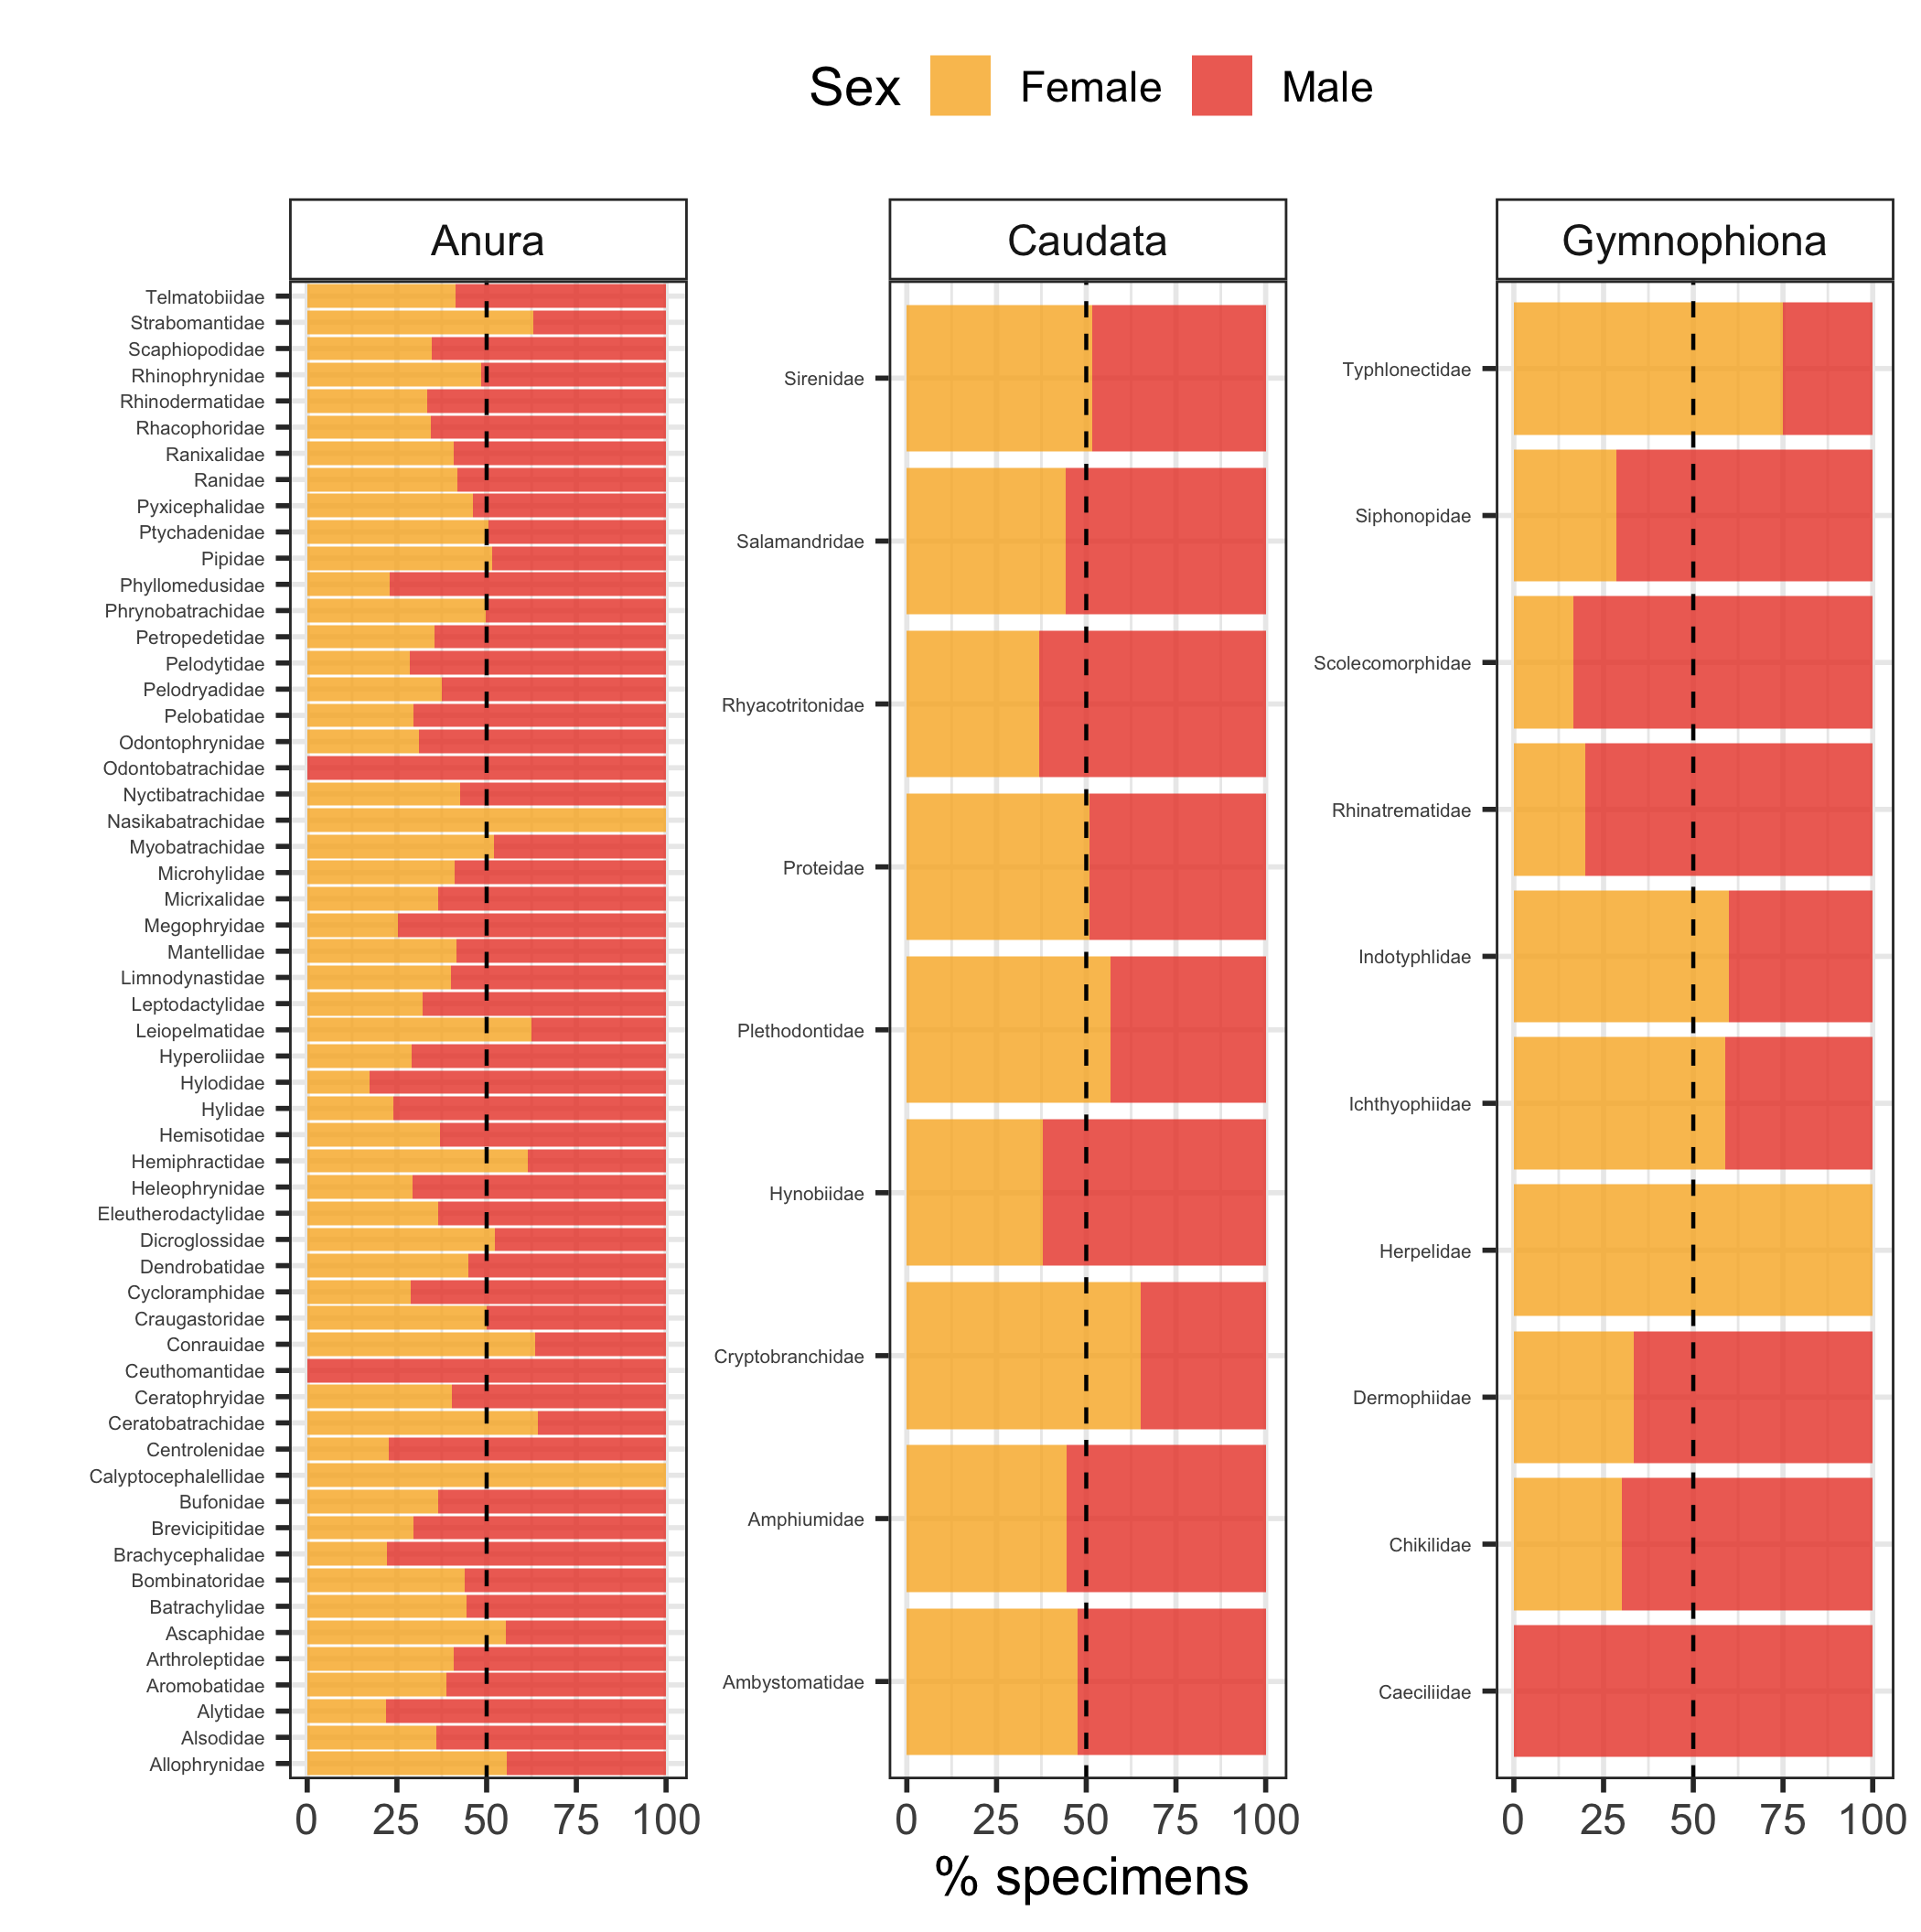
\includegraphics[width = \linewidth]{figures/all-family-amphibians.png}
  \caption{Percentages of female (yellow) and male (orange) specimen records in amphibian collections, categorised by family.
  The dashed line represents 50\% female specimens.}
  \label{fig-amphibian-family}
\end{figure}

% figure A6
\begin{figure}[H]
 \centering
  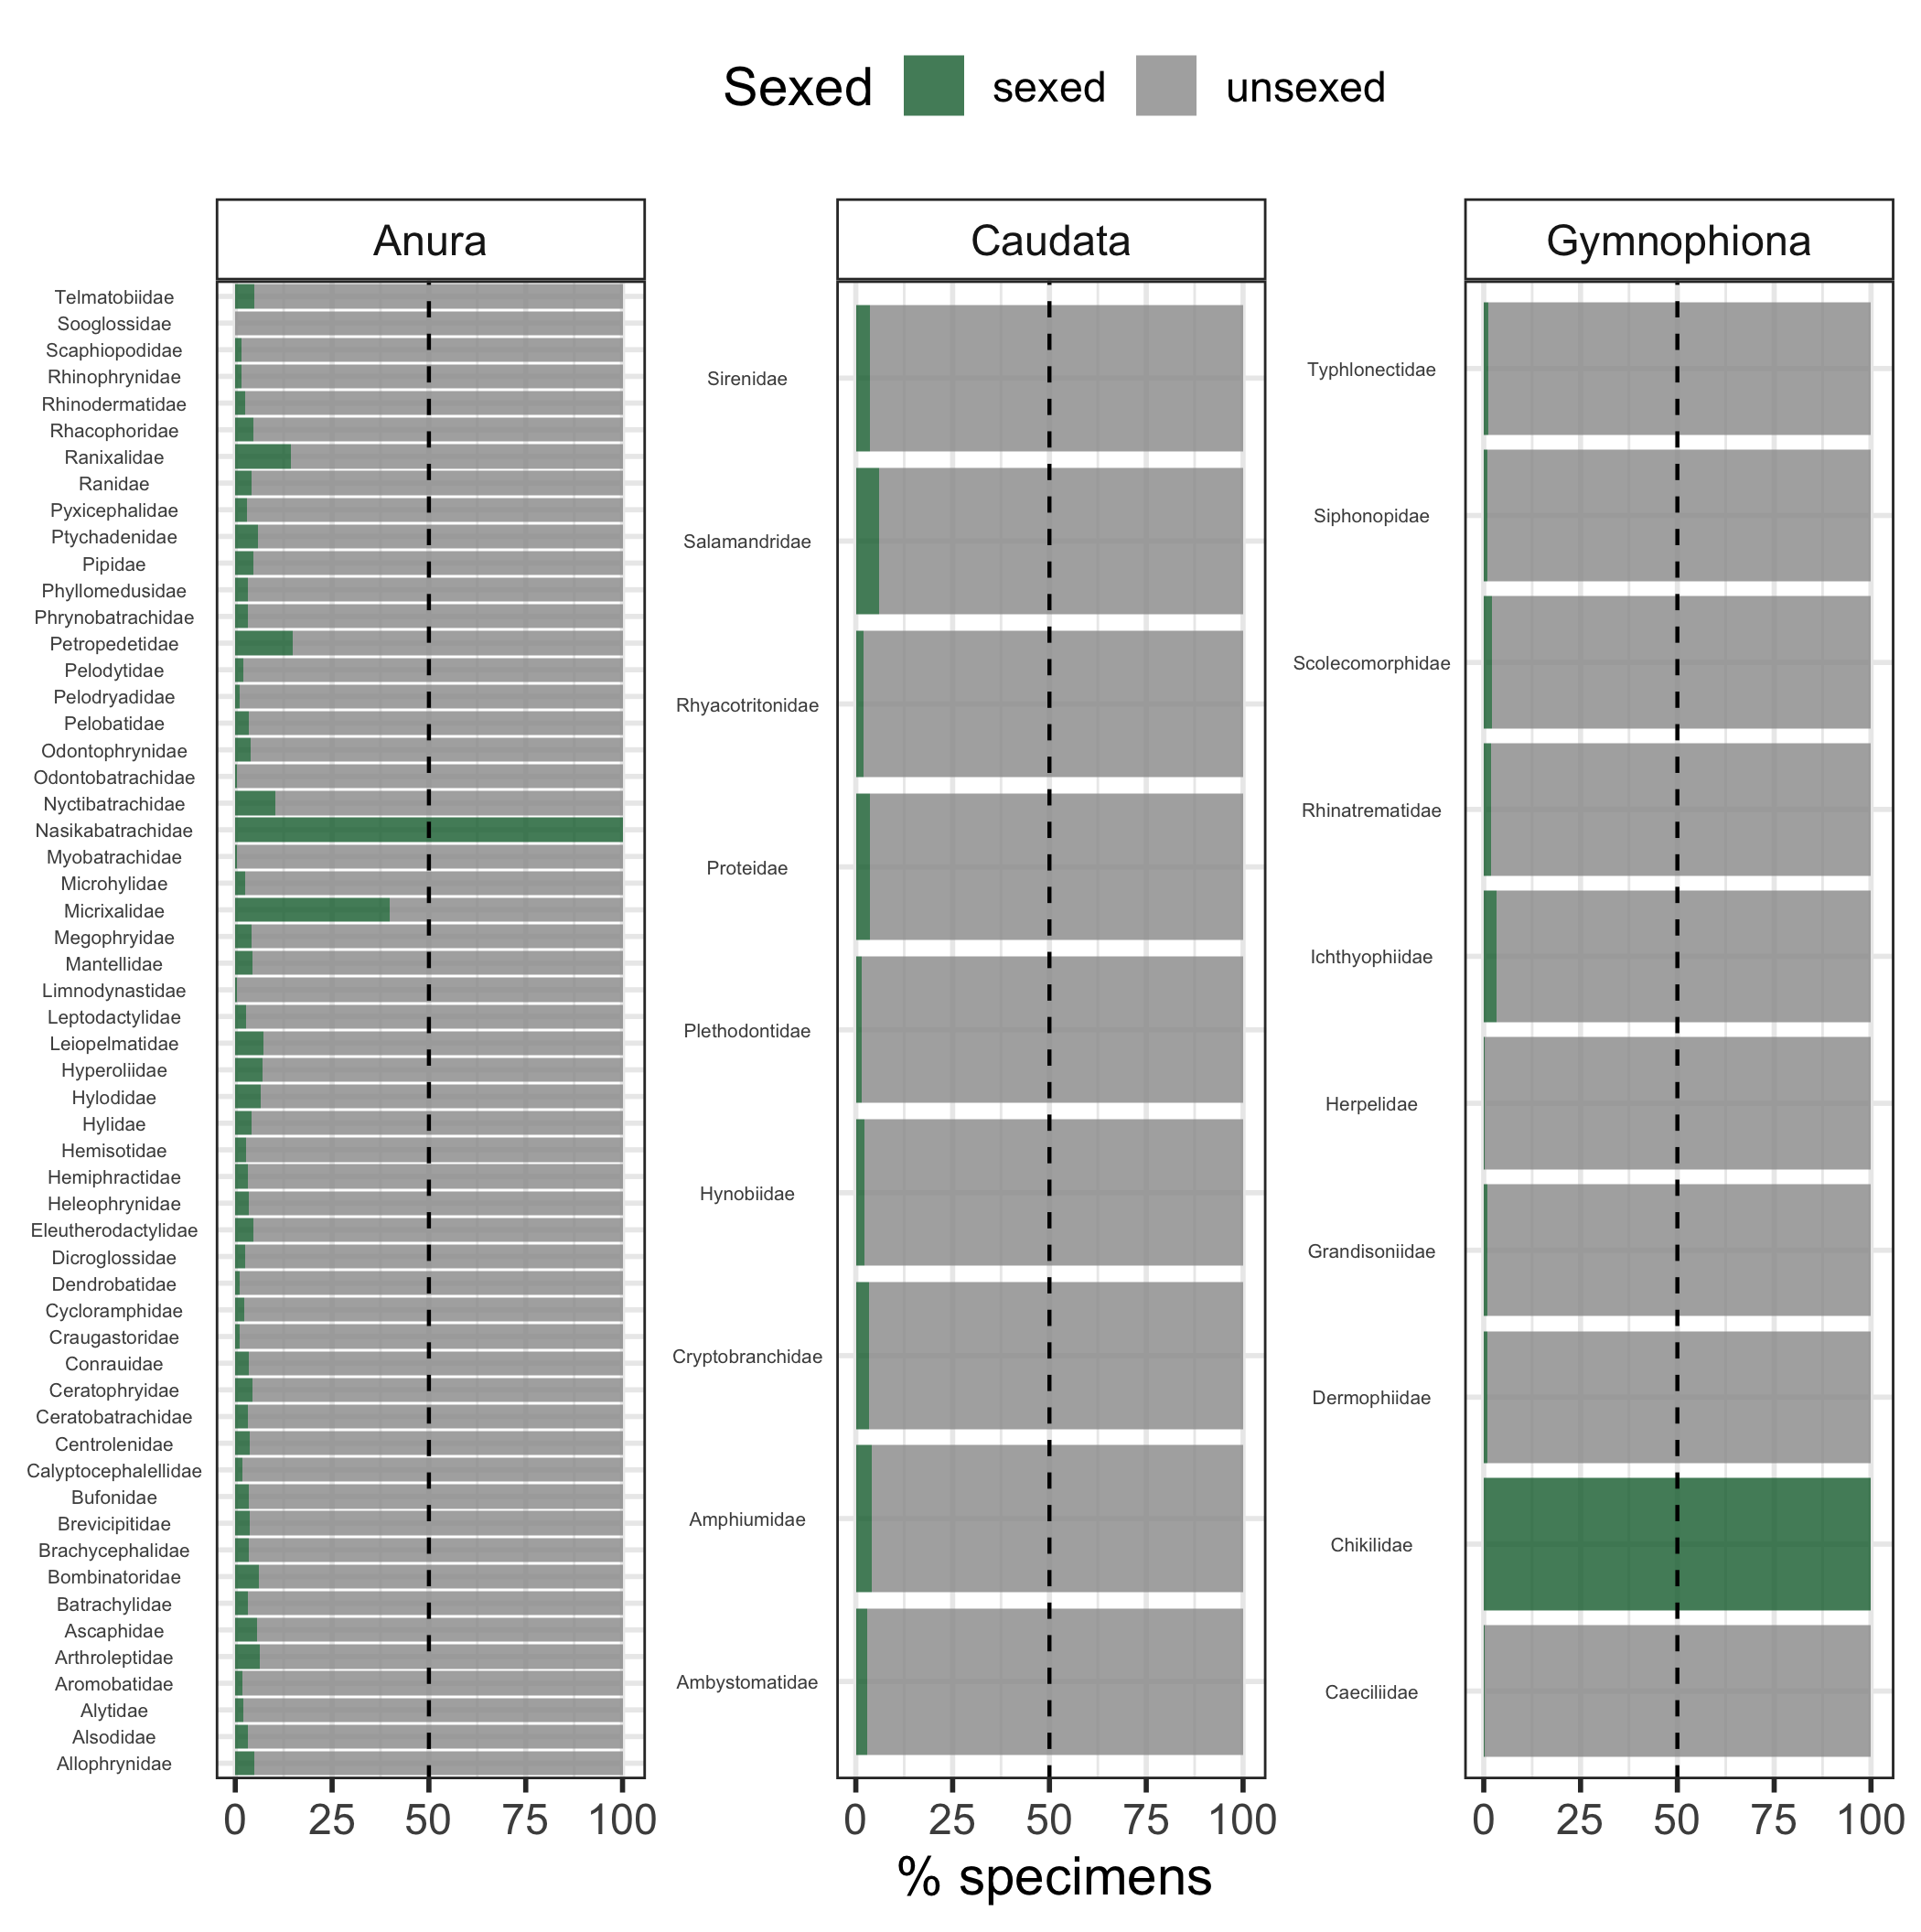
\includegraphics[width = \linewidth]{figures/all-unsexed-family-amphibians.png}
  \caption{Percentages of sexed (green) and unsexed (grey) specimen records in amphibian collections, categorised by family.
  The dashed line represents 50\% female specimens.}
  \label{fig-amphibian-family-unsexed}
\end{figure}

\newpage

\subsubsection{Reptiles}

% Table A3
% latex table generated in R 4.2.0 by xtable 1.8-4 package
% Tue Jul 26 14:18:01 2022
\begin{longtable}{llccc}
\caption{Percentages of female specimens for each family of reptiles.} \\ 
  \hline
order & family & n species & n specimens & \% female \\ 
  \hline
Crocodylia & Alligatoridae &   8 & 19536 & 50.00 \\ 
  Crocodylia & Crocodylidae &  15 & 3699 & 49.64 \\ 
  Crocodylia & Gavialidae &   1 &  18 & 50.00 \\ 
  Rhynchocephalia & Sphenodontidae &   1 &  28 & 50.00 \\ 
  Squamata & Acrochordidae &   3 & 1266 & 50.00 \\ 
  Squamata & Agamidae & 300 & 2812320 & 61.83 \\ 
  Squamata & Alopoglossidae &  11 & 2242 & 59.32 \\ 
  Squamata & Amphisbaenidae &  50 & 22348 & 49.34 \\ 
  Squamata & Anguidae &  43 & 90738 & 42.80 \\ 
  Squamata & Aniliidae &   1 &  28 & 50.00 \\ 
  Squamata & Anomalepididae &   3 &  45 & 55.56 \\ 
  Squamata & Anomochilidae &   1 &   1 & 100.00 \\ 
  Squamata & Atractaspididae &  46 & 80960 & 50.00 \\ 
  Squamata & Bipedidae &   1 &  18 & 50.00 \\ 
  Squamata & Blanidae &   1 &   1 & 100.00 \\ 
  Squamata & Boidae &  50 & 111621 & 55.26 \\ 
  Squamata & Bolyeriidae &   2 &  28 & 50.00 \\ 
  Squamata & Carphodactylidae &   7 & 370 & 56.76 \\ 
  Squamata & Chamaeleonidae & 128 & 624080 & 55.02 \\ 
  Squamata & Colubridae & 1228 & 101264527 & 53.69 \\ 
  Squamata & Cordylidae &  36 & 10962 & 59.26 \\ 
  Squamata & Corytophanidae &   9 & 9792 & 50.00 \\ 
  Squamata & Crotaphytidae &   9 & 18258 & 51.12 \\ 
  Squamata & Cyclocoridae &   5 & 856 & 50.00 \\ 
  Squamata & Cylindrophiidae &   8 & 600 & 80.00 \\ 
  Squamata & Dactyloidae & 294 & 10658097 & 61.53 \\ 
  Squamata & Dibamidae &   6 & 200 & 52.00 \\ 
  Squamata & Diplodactylidae &  56 & 26956 & 55.29 \\ 
  Squamata & Diploglossidae &  21 & 9196 & 50.00 \\ 
  Squamata & Elapidae & 227 & 1802777 & 49.39 \\ 
  Squamata & Eublepharidae &  17 & 13468 & 50.00 \\ 
  Squamata & Gekkonidae & 486 & 7536312 & 48.31 \\ 
  Squamata & Gerrhopilidae &   3 &  24 & 50.00 \\ 
  Squamata & Gerrhosauridae &  18 & 2500 & 51.00 \\ 
  Squamata & Gymnophthalmidae &  93 & 155228 & 48.64 \\ 
  Squamata & Helodermatidae &   2 & 572 & 50.00 \\ 
  Squamata & Homalopsidae &  33 & 61788 & 53.78 \\ 
  Squamata & Hoplocercidae &  11 & 2223 & 46.15 \\ 
  Squamata & Iguanidae &  36 & 101809 & 53.98 \\ 
  Squamata & Lacertidae & 209 & 2059505 & 60.14 \\ 
  Squamata & Lamprophiidae &  59 & 104838 & 50.39 \\ 
  Squamata & Lanthanotidae &   1 &   8 & 50.00 \\ 
  Squamata & Leiocephalidae &  17 & 17980 & 54.84 \\ 
  Squamata & Leiosauridae &  21 & 4488 & 48.53 \\ 
  Squamata & Leptotyphlopidae &  27 & 3842 & 50.44 \\ 
  Squamata & Liolaemidae &  90 & 148255 & 48.44 \\ 
  Squamata & Loxocemidae &   1 &  32 & 50.00 \\ 
  Squamata & Opluridae &   7 & 949 & 57.53 \\ 
  Squamata & Pareidae &  16 & 4088 & 50.00 \\ 
  Squamata & Phrynosomatidae & 138 & 5463900 & 53.85 \\ 
  Squamata & Phyllodactylidae &  56 & 52320 & 55.78 \\ 
  Squamata & Polychrotidae &   5 & 1215 & 54.81 \\ 
  Squamata & Prosymnidae &  11 & 3515 & 45.41 \\ 
  Squamata & Psammophiidae &  42 & 73470 & 58.60 \\ 
  Squamata & Pseudaspididae &   4 & 1032 & 50.00 \\ 
  Squamata & Pseudoxyrhophiidae &  59 & 57700 & 53.21 \\ 
  Squamata & Pygopodidae &   9 & 1215 & 35.80 \\ 
  Squamata & Pythonidae &  23 & 26418 & 51.99 \\ 
  Squamata & Rhineuridae &   1 &  18 & 50.00 \\ 
  Squamata & Scincidae & 467 & 8431389 & 46.19 \\ 
  Squamata & Shinisauridae &   1 &  18 & 50.00 \\ 
  Squamata & Sphaerodactylidae & 135 & 538890 & 48.14 \\ 
  Squamata & Teiidae & 109 & 1341192 & 51.70 \\ 
  Squamata & Trogonophidae &   2 &  28 & 50.00 \\ 
  Squamata & Tropidophiidae &  18 & 1664 & 50.00 \\ 
  Squamata & Tropiduridae &  81 & 172128 & 58.21 \\ 
  Squamata & Typhlopidae &  69 & 44642 & 60.86 \\ 
  Squamata & Uropeltidae &  40 & 10980 & 61.75 \\ 
  Squamata & Varanidae &  44 & 45450 & 60.73 \\ 
  Squamata & Viperidae & 192 & 3458000 & 45.04 \\ 
  Squamata & Xantusiidae &  17 & 26361 & 59.63 \\ 
  Squamata & Xenodermidae &   9 & 812 & 56.90 \\ 
  Squamata & Xenopeltidae &   2 & 114 & 55.26 \\ 
  Squamata & Xenophidiidae &   1 &   1 & 100.00 \\ 
  Squamata & Xenosauridae &   6 & 920 & 48.91 \\ 
  Testudines & Carettochelyidae &   1 &  28 & 50.00 \\ 
  Testudines & Chelidae &  45 & 233360 & 56.12 \\ 
  Testudines & Cheloniidae &   6 & 8954 & 79.73 \\ 
  Testudines & Chelydridae &   4 & 2440 & 50.00 \\ 
  Testudines & Dermatemydidae &   1 & 166 & 50.00 \\ 
  Testudines & Dermochelyidae &   1 & 276 & 50.00 \\ 
  Testudines & Emydidae &  47 & 698850 & 50.00 \\ 
  Testudines & Geoemydidae &  61 & 214475 & 55.34 \\ 
  Testudines & Kinosternidae &  22 & 251580 & 52.44 \\ 
  Testudines & Pelomedusidae &  16 & 3042 & 51.28 \\ 
  Testudines & Platysternidae &   1 &  42 & 50.00 \\ 
  Testudines & Podocnemididae &   7 & 812 & 50.00 \\ 
  Testudines & Testudinidae &  54 & 177968 & 50.72 \\ 
  Testudines & Trionychidae &  16 & 15795 & 54.70 \\ 
   \hline
\label{table-family_reptiles}
\end{longtable}


\newpage

% figure A7
\begin{figure}[H]
 \centering
  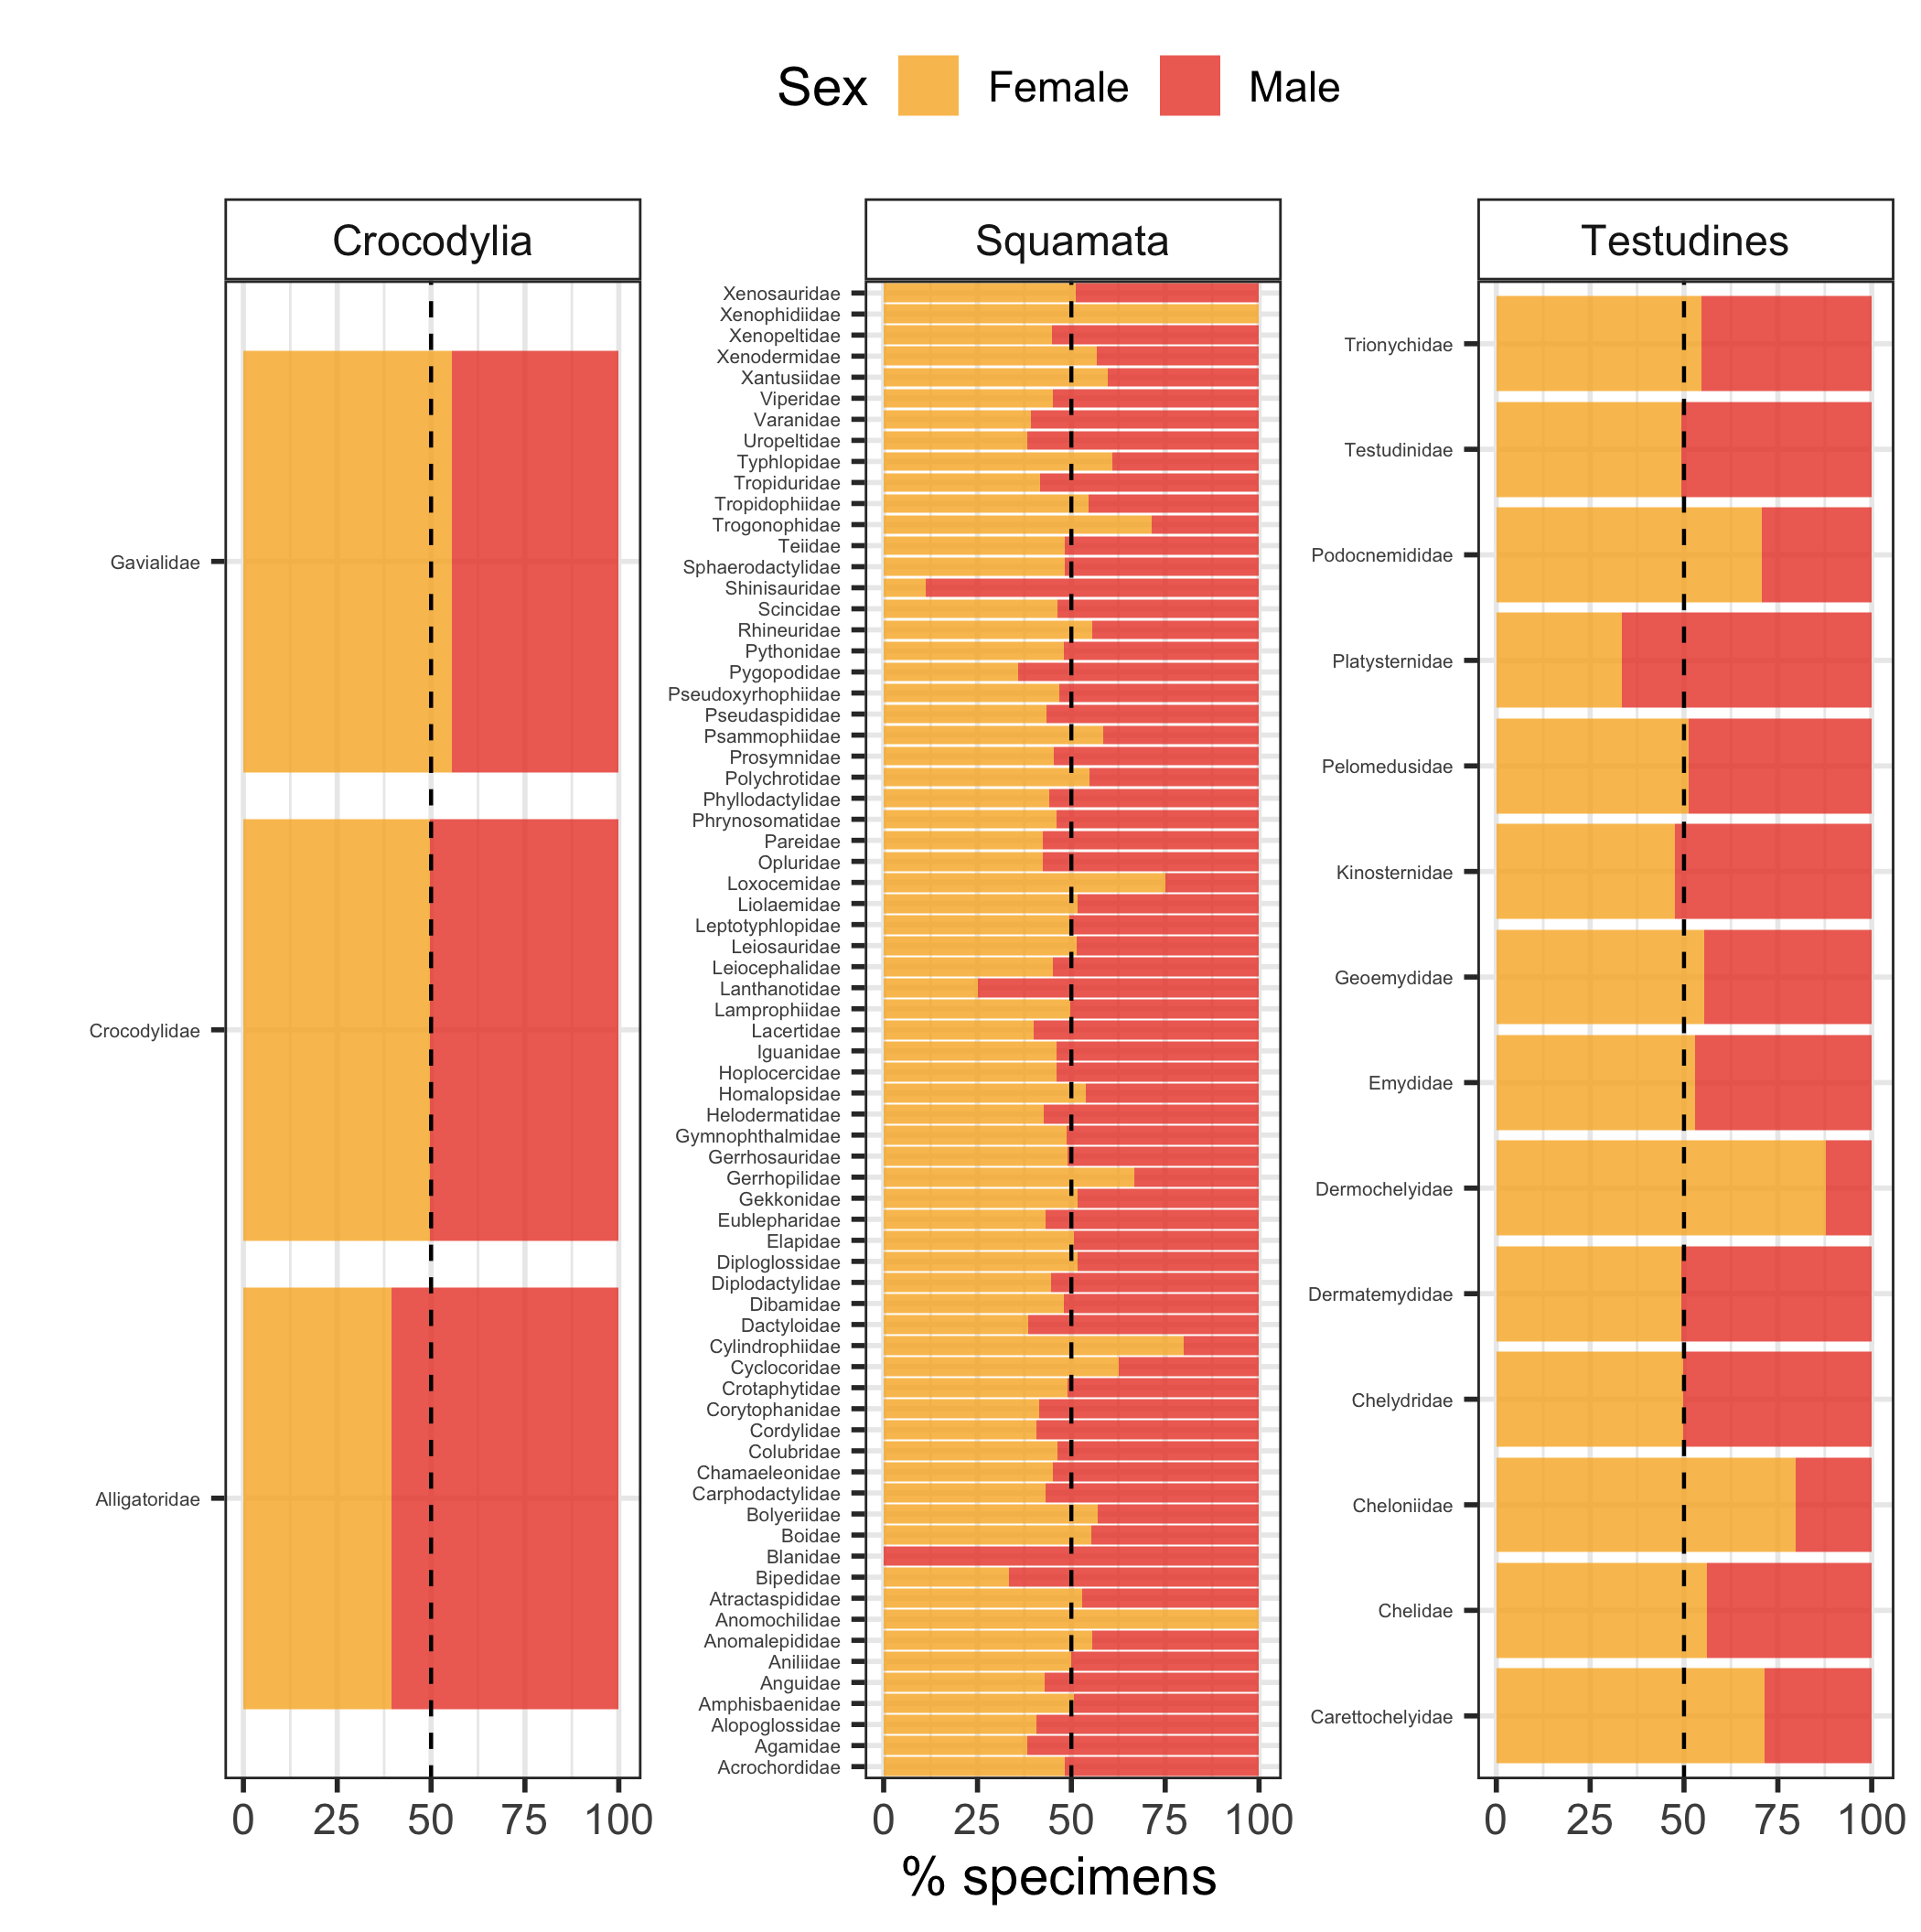
\includegraphics[width = \linewidth]{figures/all-family-reptiles.png}
  \caption{Percentages of female (yellow) and male (orange) specimen records in reptile collections, categorised by family. Rhynchocephalia is excluded as it contains only one species/family. 
  The dashed line represents 50\% female specimens.}
  \label{fig-reptile-family}
\end{figure}

% figure A8
\begin{figure}[H]
 \centering
  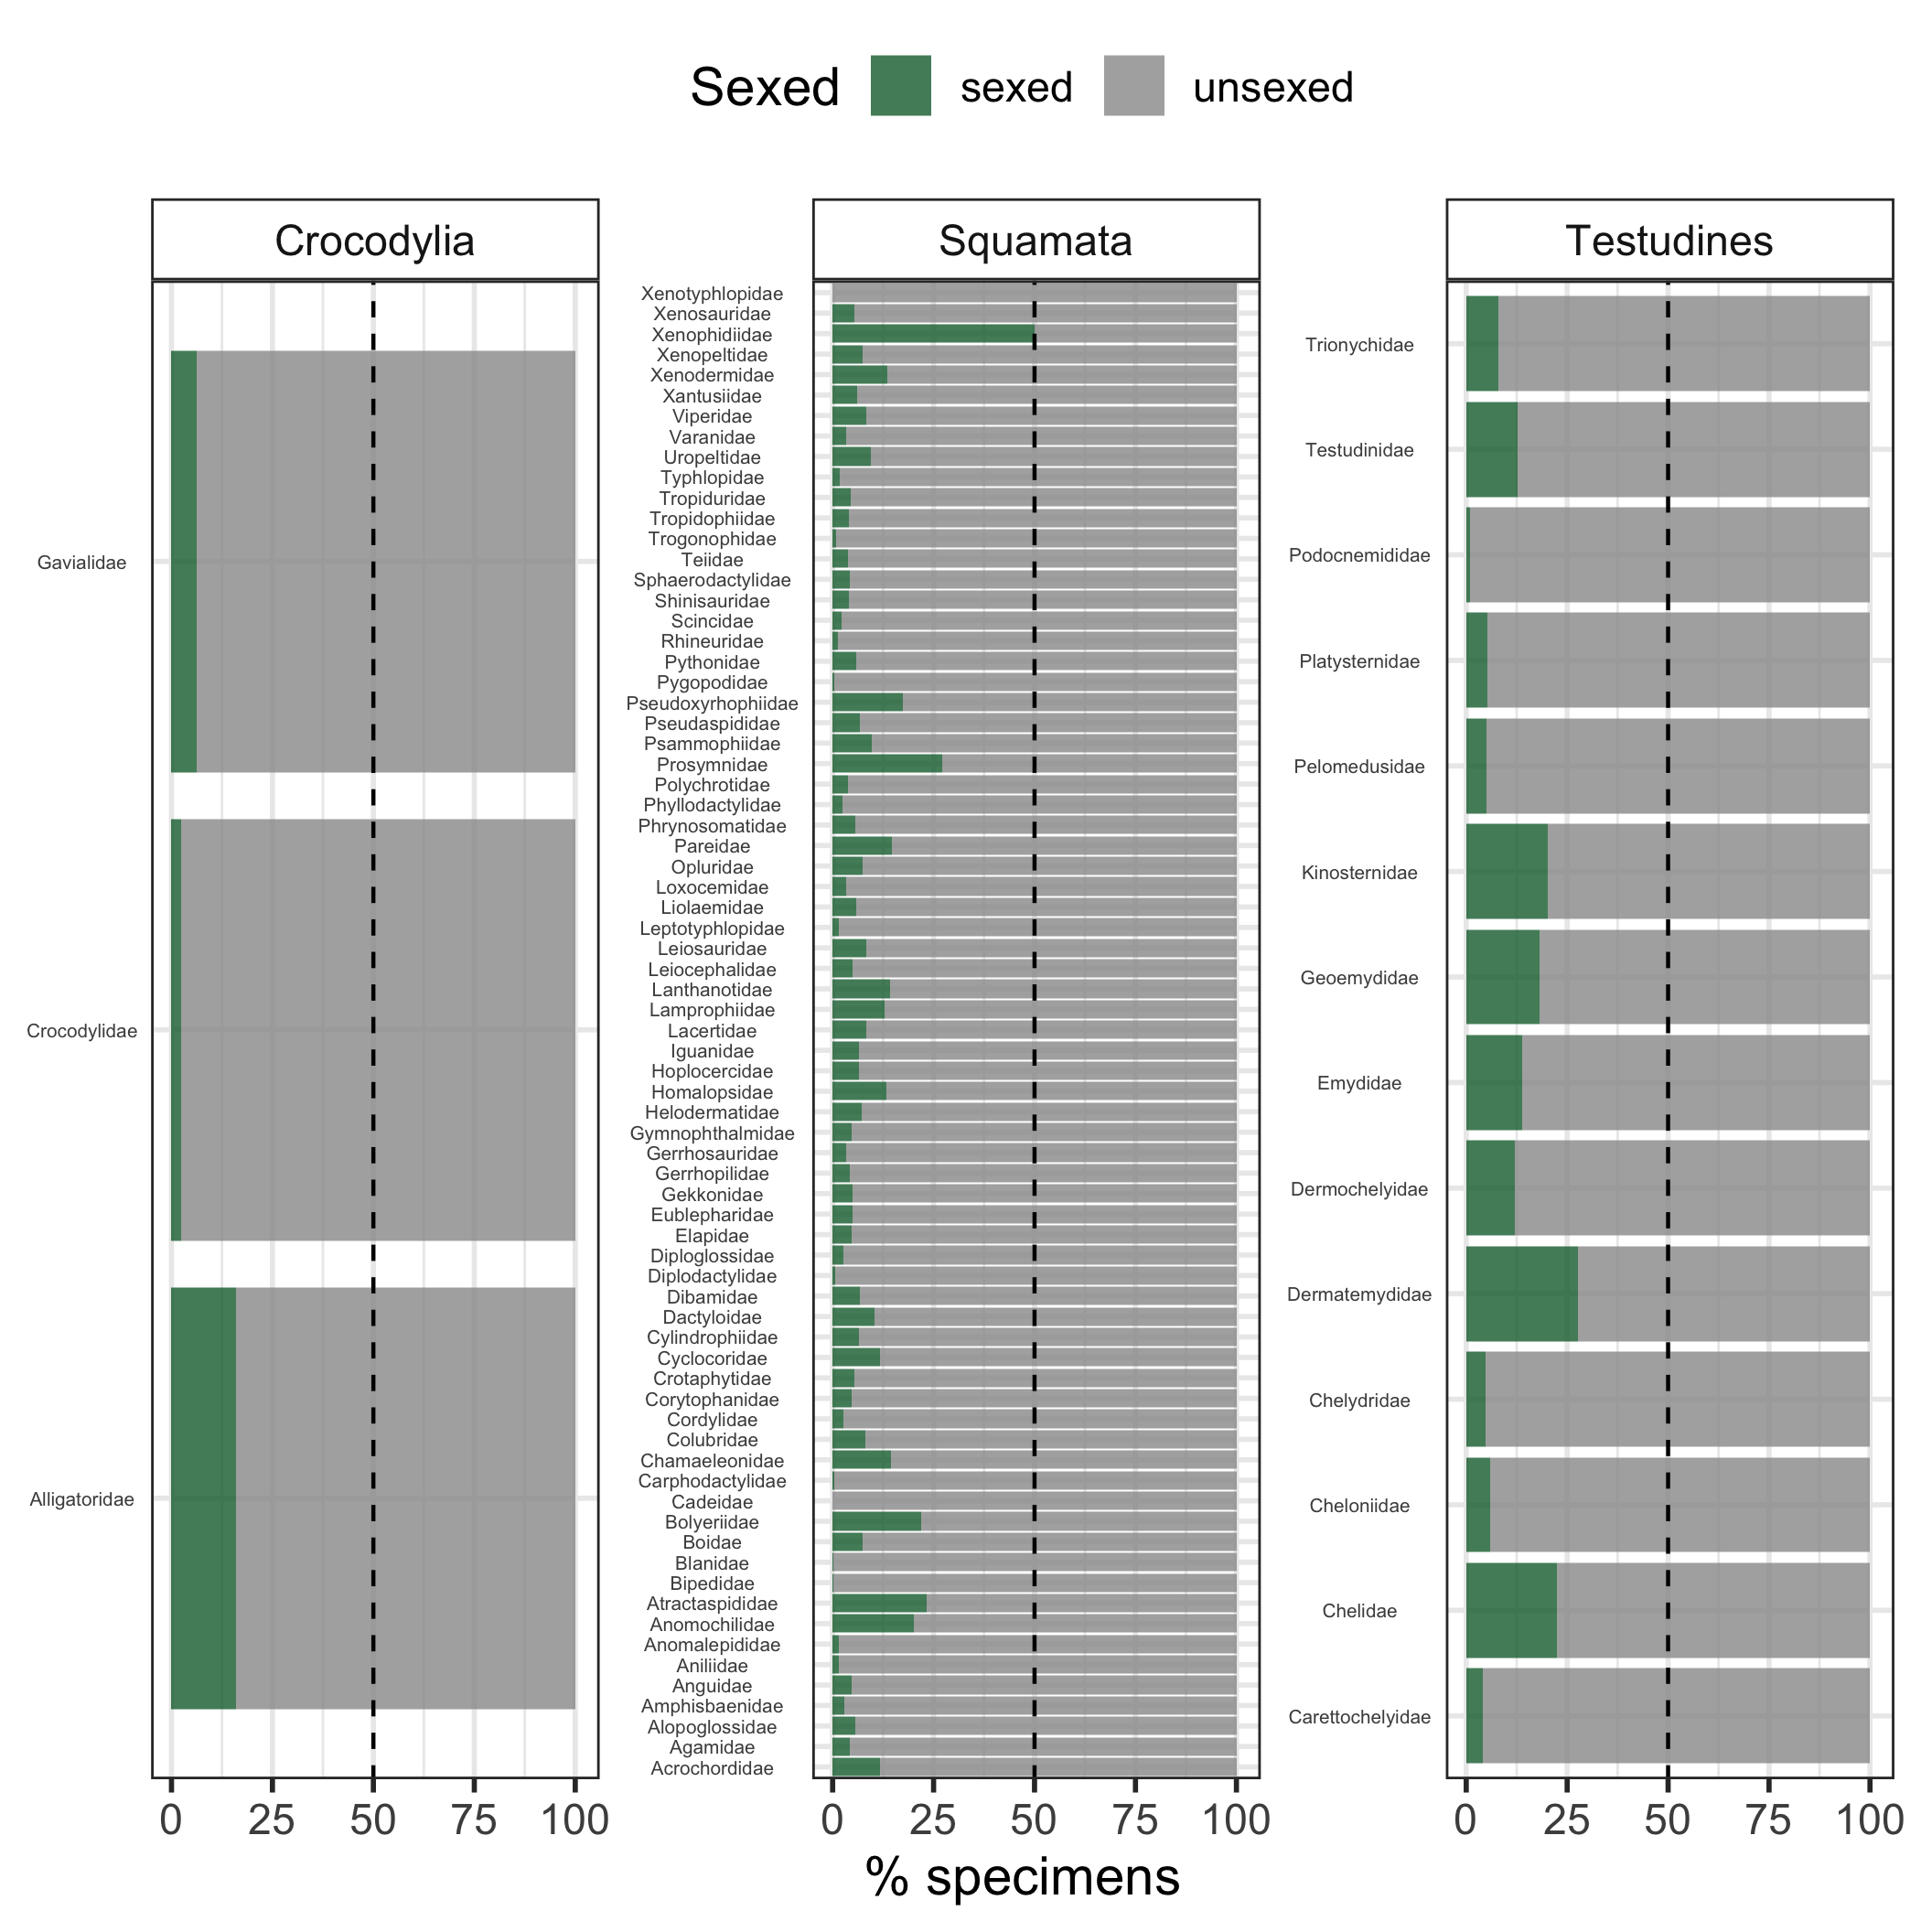
\includegraphics[width = \linewidth]{figures/all-unsexed-family-reptiles.png}
  \caption{Percentages of sexed (green) and unsexed (grey) specimen records in reptile collections, categorised by family. Rhynchocephalia is excluded as it contains only one species/family. 
  The dashed line represents 50\% female specimens.}
  \label{fig-reptile-family-unsexed}
\end{figure}



%-------------------------------------------------------------------------------
\newpage
\section{Species with the most extreme sex ratios}
%-------------------------------------------------------------------------------
% Table A4
% latex table generated in R 4.2.0 by xtable 1.8-4 package
% Tue Jul 26 14:10:22 2022
\begin{longtable}{l>{\itshape}lcc}
\caption{Amphibians and reptiles with the most extreme female-biased sex ratios
                  in our data (25 of each).} \\ 
  \hline
class & binomial & n specimens & \% female \\ 
  \hline
Amphibians & Aphantophryne sabini &  15 & 100.00 \\ 
  Amphibians & Meristogenys orphnocnemis &  13 & 100.00 \\ 
  Amphibians & Plethodon hoffmani &  53 & 100.00 \\ 
  Amphibians & Pristimantis cerasinus &  14 & 100.00 \\ 
  Amphibians & Staurois guttatus &  15 & 100.00 \\ 
  Amphibians & Staurois latopalmatus &  24 & 100.00 \\ 
  Amphibians & Nectophrynoides tornieri &  66 & 98.48 \\ 
  Amphibians & Incilius ibarrai &  37 & 97.30 \\ 
  Amphibians & Gastrotheca peruana &  33 & 96.97 \\ 
  Amphibians & Pristimantis petrobardus &  18 & 94.44 \\ 
  Amphibians & Batrachoseps wrighti &  14 & 92.86 \\ 
  Amphibians & Hyperolius substriatus &  13 & 92.31 \\ 
  Amphibians & Pristimantis dundeei &  50 & 92.00 \\ 
  Amphibians & Eleutherodactylus furcyensis &  20 & 90.00 \\ 
  Amphibians & Hylorina sylvatica &  10 & 90.00 \\ 
  Amphibians & Pristimantis chimu &  18 & 88.89 \\ 
  Amphibians & Craugastor fleischmanni &  17 & 88.24 \\ 
  Amphibians & Plethodon hubrichti &  59 & 88.14 \\ 
  Amphibians & Hemidactylium scutatum &  62 & 87.10 \\ 
  Amphibians & Chiasmocleis schubarti &  30 & 86.67 \\ 
  Amphibians & Plethodon cinereus & 926 & 84.99 \\ 
  Amphibians & Cornufer pelewensis & 400 & 84.25 \\ 
  Amphibians & Astylosternus occidentalis &  18 & 83.33 \\ 
  Amphibians & Ingerophrynus biporcatus &  12 & 83.33 \\ 
  Amphibians & Austrochaperina palmipes &  58 & 82.76 \\ 
  Reptiles & Aspidoscelis rodecki &  99 & 100.00 \\ 
  Reptiles & Brachymeles muntingkamay &  11 & 100.00 \\ 
  Reptiles & Cnemidophorus pseudolemniscatus &  43 & 100.00 \\ 
  Reptiles & Darevskia bendimahiensis &  21 & 100.00 \\ 
  Reptiles & Darevskia dahli &  43 & 100.00 \\ 
  Reptiles & Darevskia sapphirina &  26 & 100.00 \\ 
  Reptiles & Darevskia uzzelli &  25 & 100.00 \\ 
  Reptiles & Kentropyx borckiana &  12 & 100.00 \\ 
  Reptiles & Sphenomorphus forbesi &  16 & 100.00 \\ 
  Reptiles & Aspidoscelis sonorae & 325 & 99.69 \\ 
  Reptiles & Aspidoscelis neotesselatus & 197 & 98.98 \\ 
  Reptiles & Darevskia armeniaca &  81 & 98.77 \\ 
  Reptiles & Hemidactylus garnotii & 148 & 97.97 \\ 
  Reptiles & Indotyphlops braminus &  92 & 97.83 \\ 
  Reptiles & Loxopholis percarinatum &  38 & 97.37 \\ 
  Reptiles & Aspidoscelis uniparens & 164 & 95.73 \\ 
  Reptiles & Aspidoscelis exsanguis & 374 & 95.45 \\ 
  Reptiles & Lepidodactylus lugubris & 936 & 94.55 \\ 
  Reptiles & Aspidoscelis neomexicanus & 109 & 94.50 \\ 
  Reptiles & Hemiphyllodactylus typus &  16 & 93.75 \\ 
  Reptiles & Aspidoscelis velox &  46 & 93.48 \\ 
  Reptiles & Mesoclemmys nasuta &  15 & 93.33 \\ 
  Reptiles & Brachymeles bonitae &  14 & 92.86 \\ 
  Reptiles & Gymnophthalmus underwoodi &  28 & 92.86 \\ 
  Reptiles & Sphenomorphus nigrolineatus &  10 & 90.00 \\ 
   \hline
\label{table_best}
\end{longtable}


% Table A5
% latex table generated in R 4.1.0 by xtable 1.8-4 package
% Wed Aug 11 16:32:02 2021
\begin{longtable}{llcc}
\caption{Worst with >=10 specimens under 25% female} \\ 
  \hline
class & binomial & n specimens & \% female \\ 
  \hline
Amphibians & Alsodes australis &  10 & 0.00 \\ 
  Amphibians & Aplastodiscus arildae &  10 & 0.00 \\ 
  Amphibians & Aplastodiscus leucopygius &  14 & 0.00 \\ 
  Amphibians & Boana curupi &  13 & 0.00 \\ 
  Amphibians & Boana prasina &  14 & 0.00 \\ 
  Amphibians & Brachycephalus pitanga &  11 & 0.00 \\ 
  Amphibians & Dendropsophus elianeae &  12 & 0.00 \\ 
  Amphibians & Dendropsophus minusculus &  74 & 0.00 \\ 
  Amphibians & Dendropsophus pseudomeridianus &  38 & 0.00 \\ 
  Amphibians & Dendropsophus soaresi &  10 & 0.00 \\ 
  Amphibians & Eleutherodactylus eileenae &  11 & 0.00 \\ 
  Amphibians & Eleutherodactylus fuscus &  10 & 0.00 \\ 
  Amphibians & Eleutherodactylus unicolor &  10 & 0.00 \\ 
  Amphibians & Hyalinobatrachium orientale &  10 & 0.00 \\ 
  Amphibians & Hyalinobatrachium taylori &  11 & 0.00 \\ 
  Amphibians & Hyla euphorbiacea &  15 & 0.00 \\ 
  Amphibians & Hyperolius ademetzi &  14 & 0.00 \\ 
  Amphibians & Kassina fusca &  15 & 0.00 \\ 
  Amphibians & Leptopelis yaldeni &  18 & 0.00 \\ 
  Amphibians & Litoria vocivincens &  24 & 0.00 \\ 
  Amphibians & Nyctimantis brunoi &  14 & 0.00 \\ 
  Amphibians & Phrynobatrachus krefftii &  14 & 0.00 \\ 
  Amphibians & Phrynomantis annectens &  31 & 0.00 \\ 
  Amphibians & Phyllomedusa trinitatis &  11 & 0.00 \\ 
  Amphibians & Physalaemus erikae &  10 & 0.00 \\ 
  Amphibians & Physalaemus kroyeri &  13 & 0.00 \\ 
  Amphibians & Plectrohyla ixil &  12 & 0.00 \\ 
  Amphibians & Ptychohyla zophodes &  16 & 0.00 \\ 
  Amphibians & Scinax eurydice &  17 & 0.00 \\ 
  Amphibians & Scinax littoralis &  10 & 0.00 \\ 
  Amphibians & Tylototriton himalayanus &  16 & 0.00 \\ 
  Amphibians & Vitreorana eurygnatha &  10 & 0.00 \\ 
  Amphibians & Vitreorana uranoscopa &  11 & 0.00 \\ 
  Amphibians & Dendropsophus gaucheri & 121 & 1.65 \\ 
  Amphibians & Scinax alter &  51 & 1.96 \\ 
  Amphibians & Scinax boesemani &  74 & 2.70 \\ 
  Amphibians & Eleutherodactylus nitidus &  35 & 2.86 \\ 
  Amphibians & Boana polytaenia &  30 & 3.33 \\ 
  Amphibians & Aplastodiscus albosignatus &  28 & 3.57 \\ 
  Amphibians & Physalaemus ephippifer &  82 & 3.66 \\ 
  Amphibians & Breviceps gibbosus &  27 & 3.70 \\ 
  Amphibians & Boana multifasciata &  25 & 4.00 \\ 
  Amphibians & Phlyctimantis leonardi &  22 & 4.55 \\ 
  Amphibians & Phyllomedusa azurea &  21 & 4.76 \\ 
  Amphibians & Dendropsophus elegans &  61 & 4.92 \\ 
  Amphibians & Rhinella jimi &  40 & 5.00 \\ 
  Amphibians & Scinax squalirostris &  20 & 5.00 \\ 
  Amphibians & Hyperolius baumanni &  18 & 5.56 \\ 
  Amphibians & Oreolalax omeimontis &  18 & 5.56 \\ 
  Amphibians & Quasipaa spinosa &  18 & 5.56 \\ 
  Amphibians & Dendropsophus berthalutzae &  17 & 5.88 \\ 
  Amphibians & Dendropsophus oliveirai &  16 & 6.25 \\ 
  Amphibians & Pristimantis elegans &  32 & 6.25 \\ 
  Amphibians & Scinax exiguus &  16 & 6.25 \\ 
  Amphibians & Euproctus montanus &  46 & 6.52 \\ 
  Amphibians & Boana heilprini &  15 & 6.67 \\ 
  Amphibians & Boana semiguttata &  15 & 6.67 \\ 
  Amphibians & Leptobrachella oshanensis &  15 & 6.67 \\ 
  Amphibians & Leptobrachium mouhoti &  15 & 6.67 \\ 
  Amphibians & Ophryophryne hansi &  15 & 6.67 \\ 
  Amphibians & Cophixalus sphagnicola &  14 & 7.14 \\ 
  Amphibians & Hyperolius nitidulus &  54 & 7.41 \\ 
  Amphibians & Scinax fuscomarginatus &  66 & 7.58 \\ 
  Amphibians & Dendropsophus nanus & 261 & 7.66 \\ 
  Amphibians & Dendropsophus minutus & 417 & 7.67 \\ 
  Amphibians & Amolops compotrix &  13 & 7.69 \\ 
  Amphibians & Eleutherodactylus pentasyringos &  26 & 7.69 \\ 
  Amphibians & Eleutherodactylus wightmanae &  13 & 7.69 \\ 
  Amphibians & Hynobius retardatus &  26 & 7.69 \\ 
  Amphibians & Microhyla okinavensis &  26 & 7.69 \\ 
  Amphibians & Pleurodema tucumanum &  13 & 7.69 \\ 
  Amphibians & Pseudopaludicola ibisoroca &  13 & 7.69 \\ 
  Amphibians & Scinax perereca &  13 & 7.69 \\ 
  Amphibians & Boana callipleura &  12 & 8.33 \\ 
  Amphibians & Eleutherodactylus rhodesi &  12 & 8.33 \\ 
  Amphibians & Glyphoglossus yunnanensis &  12 & 8.33 \\ 
  Amphibians & Hyla annectans &  12 & 8.33 \\ 
  Amphibians & Hyloscirtus phyllognathus &  12 & 8.33 \\ 
  Amphibians & Platymantis mimulus &  12 & 8.33 \\ 
  Amphibians & Platymantis polillensis &  12 & 8.33 \\ 
  Amphibians & Rhacophorus margaritifer &  12 & 8.33 \\ 
  Amphibians & Rhinella ornata &  12 & 8.33 \\ 
  Amphibians & Sclerophrys steindachneri &  12 & 8.33 \\ 
  Amphibians & Peltophryne guentheri &  23 & 8.70 \\ 
  Amphibians & Afrixalus delicatus &  11 & 9.09 \\ 
  Amphibians & Eleutherodactylus auriculatus &  11 & 9.09 \\ 
  Amphibians & Huia cavitympanum &  33 & 9.09 \\ 
  Amphibians & Litoria freycineti &  11 & 9.09 \\ 
  Amphibians & Phyllomedusa nordestina &  11 & 9.09 \\ 
  Amphibians & Hyla andersonii & 277 & 9.39 \\ 
  Amphibians & Boana sibleszi &  42 & 9.52 \\ 
  Amphibians & Leptodactylus notoaktites &  21 & 9.52 \\ 
  Amphibians & Litoria nigropunctata &  21 & 9.52 \\ 
  Amphibians & Dendropsophus bipunctatus & 142 & 9.86 \\ 
  Amphibians & Boana riojana &  20 & 10.00 \\ 
  Amphibians & Eleutherodactylus cavernicola &  10 & 10.00 \\ 
  Amphibians & Hyperolius endjami &  20 & 10.00 \\ 
  Amphibians & Leptophryne borbonica &  10 & 10.00 \\ 
  Amphibians & Litoria prora &  10 & 10.00 \\ 
  Amphibians & Mantidactylus femoralis &  10 & 10.00 \\ 
  Amphibians & Rhacophorus bipunctatus &  10 & 10.00 \\ 
  Amphibians & Strongylopus grayii &  10 & 10.00 \\ 
  Amphibians & Teratohyla spinosa &  10 & 10.00 \\ 
  Amphibians & Xenophrys periosa &  10 & 10.00 \\ 
  Amphibians & Hyperolius lateralis &  29 & 10.34 \\ 
  Amphibians & Crossodactylus caramaschii &  67 & 10.45 \\ 
  Amphibians & Boana albomarginata & 430 & 10.47 \\ 
  Amphibians & Eleutherodactylus auriculatoides &  19 & 10.53 \\ 
  Amphibians & Hyalinobatrachium valerioi &  19 & 10.53 \\ 
  Amphibians & Pseudacris kalmi &  19 & 10.53 \\ 
  Amphibians & Hyperolius drewesi &  66 & 10.61 \\ 
  Amphibians & Amolops archotaphus &  28 & 10.71 \\ 
  Amphibians & Eleutherodactylus andrewsi &  27 & 11.11 \\ 
  Amphibians & Heleioporus albopunctatus &  18 & 11.11 \\ 
  Amphibians & Nyctimystes cheesmani &  27 & 11.11 \\ 
  Amphibians & Atelopus chiriquiensis &  35 & 11.43 \\ 
  Amphibians & Alytes obstetricans &  43 & 11.63 \\ 
  Amphibians & Brachytarsophrys intermedia &  17 & 11.76 \\ 
  Amphibians & Dendropsophus microcephalus & 136 & 11.76 \\ 
  Amphibians & Hyperolius camerunensis &  34 & 11.76 \\ 
  Amphibians & Pristimantis reichlei &  17 & 11.76 \\ 
  Amphibians & Bufotes latastii &  41 & 12.20 \\ 
  Amphibians & Atelopus spumarius &  49 & 12.24 \\ 
  Amphibians & Hyperolius quinquevittatus &  16 & 12.50 \\ 
  Amphibians & Kassina cassinoides &  16 & 12.50 \\ 
  Amphibians & Phyllomedusa camba &  16 & 12.50 \\ 
  Amphibians & Phyllomedusa vaillantii &  16 & 12.50 \\ 
  Amphibians & Rana pirica &  16 & 12.50 \\ 
  Amphibians & Pseudacris streckeri &  87 & 12.64 \\ 
  Amphibians & Dendropsophus sanborni &  38 & 13.16 \\ 
  Amphibians & Aplastodiscus perviridis &  15 & 13.33 \\ 
  Amphibians & Boana albopunctata & 120 & 13.33 \\ 
  Amphibians & Eleutherodactylus locustus &  15 & 13.33 \\ 
  Amphibians & Osteocephalus verruciger &  15 & 13.33 \\ 
  Amphibians & Platymantis browni &  30 & 13.33 \\ 
  Amphibians & Hyperolius riggenbachi &  67 & 13.43 \\ 
  Amphibians & Scinax x-signatus &  52 & 13.46 \\ 
  Amphibians & Eleutherodactylus schmidti &  37 & 13.51 \\ 
  Amphibians & Scinax fuscovarius &  37 & 13.51 \\ 
  Amphibians & Exerodonta xera &  22 & 13.64 \\ 
  Amphibians & Hyla versicolor & 440 & 13.64 \\ 
  Amphibians & Scutiger sikimmensis &  88 & 13.64 \\ 
  Amphibians & Chalcorana chalconota & 219 & 13.70 \\ 
  Amphibians & Physalaemus cuvieri & 247 & 13.77 \\ 
  Amphibians & Boana lanciformis &  29 & 13.79 \\ 
  Amphibians & Anaxyrus baxteri &  36 & 13.89 \\ 
  Amphibians & Tylototriton uyenoi &  36 & 13.89 \\ 
  Amphibians & Eleutherodactylus brevirostris &  14 & 14.29 \\ 
  Amphibians & Eleutherodactylus haitianus &  14 & 14.29 \\ 
  Amphibians & Eleutherodactylus weinlandi &  14 & 14.29 \\ 
  Amphibians & Hyla wrightorum &  21 & 14.29 \\ 
  Amphibians & Phyllomedusa tomopterna &  28 & 14.29 \\ 
  Amphibians & Pseudis bolbodactyla &  14 & 14.29 \\ 
  Amphibians & Micryletta inornata & 109 & 14.68 \\ 
  Amphibians & Buergeria buergeri &  81 & 14.81 \\ 
  Amphibians & Centrolene hesperium &  20 & 15.00 \\ 
  Amphibians & Dendropsophus bifurcus &  20 & 15.00 \\ 
  Amphibians & Anomaloglossus baeobatrachus &  26 & 15.38 \\ 
  Amphibians & Crossodactylus aeneus &  13 & 15.38 \\ 
  Amphibians & Dendropsophus acreanus &  13 & 15.38 \\ 
  Amphibians & Dendropsophus sarayacuensis &  39 & 15.38 \\ 
  Amphibians & Myersiohyla neblinaria &  13 & 15.38 \\ 
  Amphibians & Hyperolius balfouri &  19 & 15.79 \\ 
  Amphibians & Panophrys omeimontis &  19 & 15.79 \\ 
  Amphibians & Physalaemus albonotatus &  19 & 15.79 \\ 
  Amphibians & Vandijkophrynus amatolicus &  19 & 15.79 \\ 
  Amphibians & Xenopus muelleri &  57 & 15.79 \\ 
  Amphibians & Agalychnis dacnicolor &  31 & 16.13 \\ 
  Amphibians & Hyla chrysoscelis & 566 & 16.61 \\ 
  Amphibians & Boana semilineata &  12 & 16.67 \\ 
  Amphibians & Chiromantis doriae &  18 & 16.67 \\ 
  Amphibians & Eleutherodactylus alticola &  18 & 16.67 \\ 
  Amphibians & Osteopilus pulchrilineatus &  36 & 16.67 \\ 
  Amphibians & Phyllomedusa tetraploidea &  18 & 16.67 \\ 
  Amphibians & Pithecopus hypochondrialis &  84 & 16.67 \\ 
  Amphibians & Rana chaochiaoensis &  12 & 16.67 \\ 
  Amphibians & Xenopus longipes &  12 & 16.67 \\ 
  Amphibians & Phrynobatrachus gutturosus &  35 & 17.14 \\ 
  Amphibians & Desmognathus aeneus &  29 & 17.24 \\ 
  Amphibians & Tlalocohyla loquax &  29 & 17.24 \\ 
  Amphibians & Eleutherodactylus patriciae &  23 & 17.39 \\ 
  Amphibians & Eleutherodactylus portoricensis &  23 & 17.39 \\ 
  Amphibians & Tepuihyla obscura &  46 & 17.39 \\ 
  Amphibians & Eleutherodactylus cochranae &  17 & 17.65 \\ 
  Amphibians & Leptopelis ocellatus &  34 & 17.65 \\ 
  Amphibians & Meristogenys phaeomerus &  34 & 17.65 \\ 
  Amphibians & Sphaenorhynchus caramaschii &  17 & 17.65 \\ 
  Amphibians & Pseudacris nigrita & 435 & 17.70 \\ 
  Amphibians & Bombina bombina &  56 & 17.86 \\ 
  Amphibians & Hyperolius ocellatus &  89 & 17.98 \\ 
  Amphibians & Ingerophrynus celebensis & 371 & 18.06 \\ 
  Amphibians & Boana calcarata &  22 & 18.18 \\ 
  Amphibians & Dendropsophus decipiens &  11 & 18.18 \\ 
  Amphibians & Hyperolius kivuensis &  22 & 18.18 \\ 
  Amphibians & Hyperolius spinigularis &  11 & 18.18 \\ 
  Amphibians & Kaloula rigida &  11 & 18.18 \\ 
  Amphibians & Limnonectes megastomias &  11 & 18.18 \\ 
  Amphibians & Pseudacris clarkii &  22 & 18.18 \\ 
  Amphibians & Scutiger occidentalis &  66 & 18.18 \\ 
  Amphibians & Triprion petasatus &  11 & 18.18 \\ 
  Amphibians & Spea bombifrons & 115 & 18.26 \\ 
  Amphibians & Pulchrana signata & 120 & 18.33 \\ 
  Amphibians & Pseudacris brimleyi & 147 & 18.37 \\ 
  Amphibians & Ranoidea rheocola &  27 & 18.52 \\ 
  Amphibians & Odorrana hosii & 210 & 18.57 \\ 
  Amphibians & Acris gryllus & 199 & 18.59 \\ 
  Amphibians & Amolops afghanus &  48 & 18.75 \\ 
  Amphibians & Bokermannohyla hylax &  16 & 18.75 \\ 
  Amphibians & Kurixalus appendiculatus &  32 & 18.75 \\ 
  Amphibians & Phrynomantis microps &  16 & 18.75 \\ 
  Amphibians & Pseudacris brachyphona &  64 & 18.75 \\ 
  Amphibians & Rhinella magnussoni &  16 & 18.75 \\ 
  Amphibians & Semnodactylus wealii &  16 & 18.75 \\ 
  Amphibians & Pristimantis bogotensis &  53 & 18.87 \\ 
  Amphibians & Hyperolius puncticulatus & 153 & 18.95 \\ 
  Amphibians & Dendropsophus counani &  21 & 19.05 \\ 
  Amphibians & Ranoidea nannotis &  21 & 19.05 \\ 
  Amphibians & Zhangixalus omeimontis &  21 & 19.05 \\ 
  Amphibians & Dendropsophus microps &  26 & 19.23 \\ 
  Amphibians & Pelobates syriacus &  26 & 19.23 \\ 
  Amphibians & Smilisca fodiens &  26 & 19.23 \\ 
  Amphibians & Diasporus diastema &  56 & 19.64 \\ 
  Amphibians & Pseudopaludicola mystacalis & 112 & 19.64 \\ 
  Amphibians & Dendropsophus leucophyllatus &  61 & 19.67 \\ 
  Amphibians & Ambystoma macrodactylum & 121 & 19.83 \\ 
  Amphibians & Afrixalus vittiger &  15 & 20.00 \\ 
  Amphibians & Boana lemai &  15 & 20.00 \\ 
  Amphibians & Dendropsophus melanargyreus &  10 & 20.00 \\ 
  Amphibians & Hamptophryne boliviana &  10 & 20.00 \\ 
  Amphibians & Indosylvirana indica &  10 & 20.00 \\ 
  Amphibians & Leptodactylus bufonius &  50 & 20.00 \\ 
  Amphibians & Lissotriton graecus &  10 & 20.00 \\ 
  Amphibians & Pristimantis toftae &  10 & 20.00 \\ 
  Amphibians & Pseudophilautus leucorhinus &  10 & 20.00 \\ 
  Amphibians & Raorchestes chromasynchysi &  10 & 20.00 \\ 
  Amphibians & Sclerophrys langanoensis &  10 & 20.00 \\ 
  Amphibians & Sclerophrys pentoni &  15 & 20.00 \\ 
  Amphibians & Papurana celebensis &  79 & 20.25 \\ 
  Amphibians & Spea hammondii &  98 & 20.41 \\ 
  Amphibians & Eleutherodactylus pinchoni &  44 & 20.45 \\ 
  Amphibians & Hyperolius molleri &  44 & 20.45 \\ 
  Amphibians & Rana arvalis &  44 & 20.45 \\ 
  Amphibians & Rhacophorus edentulus &  44 & 20.45 \\ 
  Amphibians & Hyperolius olivaceus &  78 & 20.51 \\ 
  Amphibians & Eleutherodactylus glaphycompus &  34 & 20.59 \\ 
  Amphibians & Pseudacris triseriata & 257 & 20.62 \\ 
  Amphibians & Kassina arboricola &  29 & 20.69 \\ 
  Amphibians & Hyla avivoca &  48 & 20.83 \\ 
  Amphibians & Pseudis minuta &  24 & 20.83 \\ 
  Amphibians & Hyla japonica &  81 & 20.99 \\ 
  Amphibians & Pseudacris maculata & 257 & 21.01 \\ 
  Amphibians & Pulchrana picturata &  19 & 21.05 \\ 
  Amphibians & Ranoidea eucnemis &  19 & 21.05 \\ 
  Amphibians & Boana crepitans &  90 & 21.11 \\ 
  Amphibians & Hyla sarda &  14 & 21.43 \\ 
  Amphibians & Hyperolius concolor & 210 & 21.43 \\ 
  Amphibians & Hyperolius mosaicus &  14 & 21.43 \\ 
  Amphibians & Leptopelis christyi &  14 & 21.43 \\ 
  Amphibians & Xenopus kobeli &  14 & 21.43 \\ 
  Amphibians & Dendropsophus branneri &  51 & 21.57 \\ 
  Amphibians & Afrixalus nigeriensis &  23 & 21.74 \\ 
  Amphibians & Boana raniceps &  78 & 21.79 \\ 
  Amphibians & Hyla squirella & 876 & 21.80 \\ 
  Amphibians & Leptopelis aubryi &  73 & 21.92 \\ 
  Amphibians & Afrixalus paradorsalis &  36 & 22.22 \\ 
  Amphibians & Anaxyrus exsul &  22 & 22.73 \\ 
  Amphibians & Pseudopaludicola florencei &  22 & 22.73 \\ 
  Amphibians & Rheohyla miotympanum &  48 & 22.92 \\ 
  Amphibians & Hyperolius nasutus &  61 & 22.95 \\ 
  Amphibians & Cycloramphus boraceiensis &  13 & 23.08 \\ 
  Amphibians & Hyperolius castaneus &  13 & 23.08 \\ 
  Amphibians & Hyperolius mitchelli &  39 & 23.08 \\ 
  Amphibians & Phyllomedusa palliata &  13 & 23.08 \\ 
  Amphibians & Limnonectes microtympanum &  30 & 23.33 \\ 
  Amphibians & Atelopus hoogmoedi &  34 & 23.53 \\ 
  Amphibians & Bolitoglossa carri &  17 & 23.53 \\ 
  Amphibians & Eleutherodactylus cundalli &  34 & 23.53 \\ 
  Amphibians & Eleutherodactylus riparius &  17 & 23.53 \\ 
  Amphibians & Leptodactylus rhodomystax &  17 & 23.53 \\ 
  Amphibians & Leptopelis aubryioides &  17 & 23.53 \\ 
  Amphibians & Proceratophrys boiei &  17 & 23.53 \\ 
  Amphibians & Rana dalmatina & 136 & 23.53 \\ 
  Amphibians & Rana pyrenaica &  17 & 23.53 \\ 
  Amphibians & Sanguirana luzonensis &  85 & 23.53 \\ 
  Amphibians & Kassina cochranae &  38 & 23.68 \\ 
  Amphibians & Pseudacris crucifer & 1464 & 23.84 \\ 
  Amphibians & Eleutherodactylus nubicola &  71 & 23.94 \\ 
  Amphibians & Boana faber & 125 & 24.00 \\ 
  Amphibians & Rana kauffeldi &  25 & 24.00 \\ 
  Amphibians & Rana graeca &  54 & 24.07 \\ 
  Amphibians & Boana pardalis &  87 & 24.14 \\ 
  Amphibians & Hyperolius cinnamomeoventris &  58 & 24.14 \\ 
  Amphibians & Pseudacris feriarum & 678 & 24.19 \\ 
  Amphibians & Hoplophryne uluguruensis &  33 & 24.24 \\ 
  Amphibians & Meristogenys poecilus & 123 & 24.39 \\ 
  Amphibians & Atelopus franciscus &  28 & 25.00 \\ 
  Amphibians & Cochranella euhystrix &  12 & 25.00 \\ 
  Amphibians & Dendropsophus leali &  20 & 25.00 \\ 
  Amphibians & Eleutherodactylus lentus &  16 & 25.00 \\ 
  Amphibians & Eleutherodactylus ricordii &  12 & 25.00 \\ 
  Amphibians & Eurycea junaluska &  12 & 25.00 \\ 
  Amphibians & Leptodactylus rhodonotus &  20 & 25.00 \\ 
  Amphibians & Lithobates vibicarius &  20 & 25.00 \\ 
  Amphibians & Myersiohyla chamaeleo &  16 & 25.00 \\ 
  Amphibians & Nyctimystes kubori &  12 & 25.00 \\ 
  Amphibians & Odorrana tiannanensis &  20 & 25.00 \\ 
  Amphibians & Pleurodema brachyops &  36 & 25.00 \\ 
  Amphibians & Rana macrocnemis &  12 & 25.00 \\ 
  Amphibians & Raorchestes parvulus &  24 & 25.00 \\ 
  Amphibians & Rhinella merianae &  44 & 25.00 \\ 
  Amphibians & Scinax nebulosus &  20 & 25.00 \\ 
  Amphibians & Trichobatrachus robustus & 104 & 25.00 \\ 
  Reptiles & Anolis mccraniei &  21 & 0.00 \\ 
  Reptiles & Cryptoblepharus cursor &  13 & 0.00 \\ 
  Reptiles & Eugongylus albofasciolatus &  15 & 0.00 \\ 
  Reptiles & Myriopholis tanae &  10 & 0.00 \\ 
  Reptiles & Opisthotropis lateralis &  12 & 0.00 \\ 
  Reptiles & Podarcis lilfordi &  21 & 0.00 \\ 
  Reptiles & Ptyas fusca &  11 & 0.00 \\ 
  Reptiles & Stegonotus iridis &  10 & 0.00 \\ 
  Reptiles & Tropidophorus cocincinensis &  15 & 0.00 \\ 
  Reptiles & Emoia guttata & 103 & 0.97 \\ 
  Reptiles & Trioceros fuelleborni &  21 & 4.76 \\ 
  Reptiles & Emoia nigromarginata &  17 & 5.88 \\ 
  Reptiles & Trachylepis albilabris &  17 & 5.88 \\ 
  Reptiles & Calumma gallus &  15 & 6.67 \\ 
  Reptiles & Emoia boettgeri &  29 & 6.90 \\ 
  Reptiles & Scincella vandenburghi &  14 & 7.14 \\ 
  Reptiles & Cophoscincopus simulans &  27 & 7.41 \\ 
  Reptiles & Cryptoblepharus eximius &  36 & 8.33 \\ 
  Reptiles & Tantillita lintoni &  12 & 8.33 \\ 
  Reptiles & Varanus gouldii &  12 & 8.33 \\ 
  Reptiles & Ahaetulla fronticincta &  11 & 9.09 \\ 
  Reptiles & Alopoglossus buckleyi &  11 & 9.09 \\ 
  Reptiles & Calumma fallax &  11 & 9.09 \\ 
  Reptiles & Laticauda laticaudata &  11 & 9.09 \\ 
  Reptiles & Acanthocercus annectans &  21 & 9.52 \\ 
  Reptiles & Anolis bitectus &  10 & 10.00 \\ 
  Reptiles & Gerarda prevostiana &  10 & 10.00 \\ 
  Reptiles & Rhoptropus barnardi &  10 & 10.00 \\ 
  Reptiles & Trapelus sanguinolentus &  10 & 10.00 \\ 
  Reptiles & Kinyongia multituberculata &  86 & 10.47 \\ 
  Reptiles & Hemidactylus leschenaultii &  19 & 10.53 \\ 
  Reptiles & Anolis brevirostris & 122 & 10.66 \\ 
  Reptiles & Caiman latirostris &  18 & 11.11 \\ 
  Reptiles & Thamnodynastes pallidus &  18 & 11.11 \\ 
  Reptiles & Ptyas multicincta &  17 & 11.76 \\ 
  Reptiles & Sonora palarostris &  34 & 11.76 \\ 
  Reptiles & Draco formosus &  33 & 12.12 \\ 
  Reptiles & Aspidoscelis maximus &  16 & 12.50 \\ 
  Reptiles & Leiocephalus barahonensis &  16 & 12.50 \\ 
  Reptiles & Acanthodactylus bedriagai &  23 & 13.04 \\ 
  Reptiles & Anolis cooki &  30 & 13.33 \\ 
  Reptiles & Podarcis melisellensis &  50 & 14.00 \\ 
  Reptiles & Anolis crassulus &  21 & 14.29 \\ 
  Reptiles & Anolis cupreus &  21 & 14.29 \\ 
  Reptiles & Perochirus ateles &  35 & 14.29 \\ 
  Reptiles & Pholidoscelis taeniurus &  21 & 14.29 \\ 
  Reptiles & Stenocercus guentheri &  14 & 14.29 \\ 
  Reptiles & Afrotyphlops congestus &  20 & 15.00 \\ 
  Reptiles & Chalarodon madagascariensis &  20 & 15.00 \\ 
  Reptiles & Calotes mystaceus &  33 & 15.15 \\ 
  Reptiles & Abronia deppii &  13 & 15.38 \\ 
  Reptiles & Acanthodactylus pardalis &  13 & 15.38 \\ 
  Reptiles & Anolis caudalis &  19 & 15.79 \\ 
  Reptiles & Draco haematopogon &  44 & 15.91 \\ 
  Reptiles & Acanthocercus adramitanus &  18 & 16.67 \\ 
  Reptiles & Anolis nelsoni &  12 & 16.67 \\ 
  Reptiles & Colobosaura modesta &  12 & 16.67 \\ 
  Reptiles & Diploderma swinhonis &  24 & 16.67 \\ 
  Reptiles & Liolaemus lemniscatus &  12 & 16.67 \\ 
  Reptiles & Micrurus hemprichii &  12 & 16.67 \\ 
  Reptiles & Panaspis breviceps &  12 & 16.67 \\ 
  Reptiles & Tropidophorus grayi &  18 & 16.67 \\ 
  Reptiles & Lachesis muta &  23 & 17.39 \\ 
  Reptiles & Oligodon cyclurus &  23 & 17.39 \\ 
  Reptiles & Anolis ricordii &  28 & 17.86 \\ 
  Reptiles & Perochirus scutellatus &  28 & 17.86 \\ 
  Reptiles & Uromastyx acanthinura &  28 & 17.86 \\ 
  Reptiles & Acanthodactylus schmidti &  11 & 18.18 \\ 
  Reptiles & Anolis rimarum &  11 & 18.18 \\ 
  Reptiles & Crotaphytus dickersonae &  11 & 18.18 \\ 
  Reptiles & Geophis hoffmanni &  11 & 18.18 \\ 
  Reptiles & Mastigodryas dorsalis &  22 & 18.18 \\ 
  Reptiles & Philochortus hardeggeri &  11 & 18.18 \\ 
  Reptiles & Protobothrops mucrosquamatus &  44 & 18.18 \\ 
  Reptiles & Pseudoboodon lemniscatus &  11 & 18.18 \\ 
  Reptiles & Ptyas dhumnades &  11 & 18.18 \\ 
  Reptiles & Sauromalus varius &  11 & 18.18 \\ 
  Reptiles & Takydromus sexlineatus &  60 & 18.33 \\ 
  Reptiles & Algyroides fitzingeri &  16 & 18.75 \\ 
  Reptiles & Algyroides nigropunctatus &  16 & 18.75 \\ 
  Reptiles & Karusasaurus polyzonus &  16 & 18.75 \\ 
  Reptiles & Anolis luteosignifer & 330 & 18.79 \\ 
  Reptiles & Anolis tropidonotus &  69 & 18.84 \\ 
  Reptiles & Aspidoscelis lineattissimus &  53 & 18.87 \\ 
  Reptiles & Emoia impar & 233 & 18.88 \\ 
  Reptiles & Aprasia repens &  21 & 19.05 \\ 
  Reptiles & Pachydactylus rangei &  21 & 19.05 \\ 
  Reptiles & Pedioplanis namaquensis &  42 & 19.05 \\ 
  Reptiles & Anolis longitibialis &  26 & 19.23 \\ 
  Reptiles & Anolis allisoni &  36 & 19.44 \\ 
  Reptiles & Calotes emma &  51 & 19.61 \\ 
  Reptiles & Anolis pachypus &  10 & 20.00 \\ 
  Reptiles & Calotes jerdoni &  10 & 20.00 \\ 
  Reptiles & Darevskia rudis &  10 & 20.00 \\ 
  Reptiles & Dendrelaphis gastrostictus &  10 & 20.00 \\ 
  Reptiles & Eirenis decemlineatus &  10 & 20.00 \\ 
  Reptiles & Elapsoidea sundevallii &  10 & 20.00 \\ 
  Reptiles & Eremias dzungarica &  10 & 20.00 \\ 
  Reptiles & Petracola ventrimaculatus &  10 & 20.00 \\ 
  Reptiles & Psammodromus edwarsianus &  15 & 20.00 \\ 
  Reptiles & Psammophis lineolatus &  10 & 20.00 \\ 
  Reptiles & Rhadinaea decorata &  40 & 20.00 \\ 
  Reptiles & Sceloporus heterolepis &  10 & 20.00 \\ 
  Reptiles & Spilotes sulphureus &  20 & 20.00 \\ 
  Reptiles & Stegonotus guentheri &  10 & 20.00 \\ 
  Reptiles & Stegonotus heterurus &  10 & 20.00 \\ 
  Reptiles & Uropeltis ceylanica &  10 & 20.00 \\ 
  Reptiles & Varanus salvadorii &  10 & 20.00 \\ 
  Reptiles & Xylophis perroteti &  10 & 20.00 \\ 
  Reptiles & Pholidoscelis chrysolaemus &  44 & 20.45 \\ 
  Reptiles & Anolis matudai &  24 & 20.83 \\ 
  Reptiles & Eremias persica &  24 & 20.83 \\ 
  Reptiles & Anolis websteri &  19 & 21.05 \\ 
  Reptiles & Caledoniscincus atropunctatus &  38 & 21.05 \\ 
  Reptiles & Thamnophis nigronuchalis &  19 & 21.05 \\ 
  Reptiles & Anolis aeneus &  52 & 21.15 \\ 
  Reptiles & Anolis oculatus & 118 & 21.19 \\ 
  Reptiles & Ophisaurus ventralis & 141 & 21.28 \\ 
  Reptiles & Amphibolurus muricatus &  14 & 21.43 \\ 
  Reptiles & Kinosternon acutum &  14 & 21.43 \\ 
  Reptiles & Melanosuchus niger &  14 & 21.43 \\ 
  Reptiles & Sphenodon punctatus &  14 & 21.43 \\ 
  Reptiles & Stenodactylus doriae &  14 & 21.43 \\ 
  Reptiles & Takydromus dorsalis &  14 & 21.43 \\ 
  Reptiles & Tantilla vulcani &  14 & 21.43 \\ 
  Reptiles & Gehyra dubia &  23 & 21.74 \\ 
  Reptiles & Acanthosaura lepidogaster &  41 & 21.95 \\ 
  Reptiles & Trimeresurus stejnegeri &  91 & 21.98 \\ 
  Reptiles & Draco sumatranus & 163 & 22.09 \\ 
  Reptiles & Acanthodactylus maculatus &  36 & 22.22 \\ 
  Reptiles & Crenadactylus ocellatus &  18 & 22.22 \\ 
  Reptiles & Erythrolamprus mimus &  18 & 22.22 \\ 
  Reptiles & Gonatodes ocellatus &  18 & 22.22 \\ 
  Reptiles & Scincella reevesii &  31 & 22.58 \\ 
  Reptiles & Anolis pulchellus & 113 & 23.01 \\ 
  Reptiles & Ailuronyx seychellensis &  13 & 23.08 \\ 
  Reptiles & Anolis scypheus &  39 & 23.08 \\ 
  Reptiles & Chlamydosaurus kingii &  13 & 23.08 \\ 
  Reptiles & Kinosternon angustipons &  13 & 23.08 \\ 
  Reptiles & Latastia boscai &  13 & 23.08 \\ 
  Reptiles & Microlophus peruvianus &  26 & 23.08 \\ 
  Reptiles & Tretioscincus agilis &  26 & 23.08 \\ 
  Reptiles & Xenelaphis hexagonotus &  13 & 23.08 \\ 
  Reptiles & Zamenis longissimus &  26 & 23.08 \\ 
  Reptiles & Zamenis situla &  13 & 23.08 \\ 
  Reptiles & Sonora occipitalis & 112 & 23.21 \\ 
  Reptiles & Calamaria septentrionalis &  30 & 23.33 \\ 
  Reptiles & Nucras boulengeri &  30 & 23.33 \\ 
  Reptiles & Phrynocephalus theobaldi &  17 & 23.53 \\ 
  Reptiles & Cnemidophorus murinus &  42 & 23.81 \\ 
  Reptiles & Lygodactylus gutturalis &  21 & 23.81 \\ 
  Reptiles & Pseudopus apodus &  21 & 23.81 \\ 
  Reptiles & Acanthocercus atricollis & 125 & 24.00 \\ 
  Reptiles & Acanthodactylus boskianus & 175 & 24.00 \\ 
  Reptiles & Trimerodytes percarinatus &  25 & 24.00 \\ 
  Reptiles & Xantusia bezyi &  25 & 24.00 \\ 
  Reptiles & Mastigodryas melanolomus &  95 & 24.21 \\ 
  Reptiles & Pachydactylus punctatus &  33 & 24.24 \\ 
  Reptiles & Trachemys stejnegeri &  41 & 24.39 \\ 
  Reptiles & Anolis semilineatus &  49 & 24.49 \\ 
  Reptiles & Sphaerodactylus fantasticus &  57 & 24.56 \\ 
  Reptiles & Anolis aliniger &  20 & 25.00 \\ 
  Reptiles & Anolis wattsii &  44 & 25.00 \\ 
  Reptiles & Bothrops alternatus &  24 & 25.00 \\ 
  Reptiles & Corytophanes cristatus &  56 & 25.00 \\ 
  Reptiles & Crotaphopeltis degeni &  12 & 25.00 \\ 
  Reptiles & Cuora trifasciata &  20 & 25.00 \\ 
  Reptiles & Draco jareckii &  16 & 25.00 \\ 
  Reptiles & Drymoluber dichrous &  24 & 25.00 \\ 
  Reptiles & Helicops pastazae &  28 & 25.00 \\ 
  Reptiles & Homopholis walbergii &  12 & 25.00 \\ 
  Reptiles & Ichnotropis capensis &  24 & 25.00 \\ 
  Reptiles & Japalura tricarinata &  32 & 25.00 \\ 
  Reptiles & Kinyongia fischeri &  84 & 25.00 \\ 
  Reptiles & Liolaemus orientalis &  12 & 25.00 \\ 
  Reptiles & Lycodon laoensis &  16 & 25.00 \\ 
  Reptiles & Micrurus altirostris &  16 & 25.00 \\ 
  Reptiles & Ophisops jerdonii &  16 & 25.00 \\ 
  Reptiles & Phelsuma lineata &  20 & 25.00 \\ 
  Reptiles & Pholidoscelis griswoldi &  16 & 25.00 \\ 
  Reptiles & Phrynops hilarii &  16 & 25.00 \\ 
  Reptiles & Physignathus cocincinus &  20 & 25.00 \\ 
  Reptiles & Plestiodon brevirostris &  28 & 25.00 \\ 
  Reptiles & Podarcis pityusensis &  12 & 25.00 \\ 
  Reptiles & Pseudechis porphyriacus &  12 & 25.00 \\ 
  Reptiles & Rhabdophis nuchalis &  48 & 25.00 \\ 
  Reptiles & Rhadinaea laureata &  16 & 25.00 \\ 
  Reptiles & Sceloporus angustus &  20 & 25.00 \\ 
  Reptiles & Sitana ponticeriana &  20 & 25.00 \\ 
  Reptiles & Tropidodipsas fischeri &  20 & 25.00 \\ 
  Reptiles & Varzea altamazonica &  16 & 25.00 \\ 
   \hline
\hline
\label{table-best}
\end{longtable}


%-------------------------------------------------------------------------------
\newpage
\section{Numbers of species in each analysis}
%-------------------------------------------------------------------------------

\begin{table}[H]
\centering
\begin{tabular}{lcccc}

  \hline
  \textbf{Model} & \textbf{Sexed only} & \textbf{All specimens}\\ 
  \hline
  \textbf{AMPHIBIANS} & &\\
  \hline
  orders & 1143 & 4818\\
  years & 1300 & 34320\\
  max size & 229 & 232\\
  female size & 181 & 184\\
  male size & 181 & 184\\
  SSD & 175 & 178\\
  larger sex & 195 & 198\\
  \hline
  \textbf{REPTILES} & &\\
  \hline
  orders & 2163 & 6727\\
  years & 2816 & 44054\\
  max size & 305 & 308\\
  female size & 197 & 198\\
  male size & 175 & 177\\
  SSD & 162 & 163\\
  larger sex & 235 & 236\\
  \hline

\label{table_numbers}
\end{tabular}
\caption{Numbers of species in each of our models, investigating males and females (sexed only) and sexed and unsexed (all specimens). Numbers in years analyses are species x year combinations. SSD is sexual size dimorphism. All species have order data.} 

\end{table}

%-------------------------------------------------------------------------------
\newpage
\section{More inclusive taxonomic groupings for Squamata}
%-------------------------------------------------------------------------------
%% latex table generated in R 4.2.0 by xtable 1.8-4 package
% Tue Jul 26 14:10:22 2022
\begin{longtable}{l>{\itshape}lcc}
\caption{Amphibians and reptiles with the most extreme female-biased sex ratios
                  in our data (25 of each).} \\ 
  \hline
class & binomial & n specimens & \% female \\ 
  \hline
Amphibians & Aphantophryne sabini &  15 & 100.00 \\ 
  Amphibians & Meristogenys orphnocnemis &  13 & 100.00 \\ 
  Amphibians & Plethodon hoffmani &  53 & 100.00 \\ 
  Amphibians & Pristimantis cerasinus &  14 & 100.00 \\ 
  Amphibians & Staurois guttatus &  15 & 100.00 \\ 
  Amphibians & Staurois latopalmatus &  24 & 100.00 \\ 
  Amphibians & Nectophrynoides tornieri &  66 & 98.48 \\ 
  Amphibians & Incilius ibarrai &  37 & 97.30 \\ 
  Amphibians & Gastrotheca peruana &  33 & 96.97 \\ 
  Amphibians & Pristimantis petrobardus &  18 & 94.44 \\ 
  Amphibians & Batrachoseps wrighti &  14 & 92.86 \\ 
  Amphibians & Hyperolius substriatus &  13 & 92.31 \\ 
  Amphibians & Pristimantis dundeei &  50 & 92.00 \\ 
  Amphibians & Eleutherodactylus furcyensis &  20 & 90.00 \\ 
  Amphibians & Hylorina sylvatica &  10 & 90.00 \\ 
  Amphibians & Pristimantis chimu &  18 & 88.89 \\ 
  Amphibians & Craugastor fleischmanni &  17 & 88.24 \\ 
  Amphibians & Plethodon hubrichti &  59 & 88.14 \\ 
  Amphibians & Hemidactylium scutatum &  62 & 87.10 \\ 
  Amphibians & Chiasmocleis schubarti &  30 & 86.67 \\ 
  Amphibians & Plethodon cinereus & 926 & 84.99 \\ 
  Amphibians & Cornufer pelewensis & 400 & 84.25 \\ 
  Amphibians & Astylosternus occidentalis &  18 & 83.33 \\ 
  Amphibians & Ingerophrynus biporcatus &  12 & 83.33 \\ 
  Amphibians & Austrochaperina palmipes &  58 & 82.76 \\ 
  Reptiles & Aspidoscelis rodecki &  99 & 100.00 \\ 
  Reptiles & Brachymeles muntingkamay &  11 & 100.00 \\ 
  Reptiles & Cnemidophorus pseudolemniscatus &  43 & 100.00 \\ 
  Reptiles & Darevskia bendimahiensis &  21 & 100.00 \\ 
  Reptiles & Darevskia dahli &  43 & 100.00 \\ 
  Reptiles & Darevskia sapphirina &  26 & 100.00 \\ 
  Reptiles & Darevskia uzzelli &  25 & 100.00 \\ 
  Reptiles & Kentropyx borckiana &  12 & 100.00 \\ 
  Reptiles & Sphenomorphus forbesi &  16 & 100.00 \\ 
  Reptiles & Aspidoscelis sonorae & 325 & 99.69 \\ 
  Reptiles & Aspidoscelis neotesselatus & 197 & 98.98 \\ 
  Reptiles & Darevskia armeniaca &  81 & 98.77 \\ 
  Reptiles & Hemidactylus garnotii & 148 & 97.97 \\ 
  Reptiles & Indotyphlops braminus &  92 & 97.83 \\ 
  Reptiles & Loxopholis percarinatum &  38 & 97.37 \\ 
  Reptiles & Aspidoscelis uniparens & 164 & 95.73 \\ 
  Reptiles & Aspidoscelis exsanguis & 374 & 95.45 \\ 
  Reptiles & Lepidodactylus lugubris & 936 & 94.55 \\ 
  Reptiles & Aspidoscelis neomexicanus & 109 & 94.50 \\ 
  Reptiles & Hemiphyllodactylus typus &  16 & 93.75 \\ 
  Reptiles & Aspidoscelis velox &  46 & 93.48 \\ 
  Reptiles & Mesoclemmys nasuta &  15 & 93.33 \\ 
  Reptiles & Brachymeles bonitae &  14 & 92.86 \\ 
  Reptiles & Gymnophthalmus underwoodi &  28 & 92.86 \\ 
  Reptiles & Sphenomorphus nigrolineatus &  10 & 90.00 \\ 
   \hline
\label{table_best}
\end{longtable}


\begin{longtable}{lll}
\caption{} 

\hline
\textbf{Family} & \textbf{Grouping 1} & \textbf{Grouping 2}\\ 
\hline
Anguidae & Anguiformes & Anguiformes \\
Diploglossidae & Anguiformes & Anguiformes \\
Helodermatidae & Anguiformes & Anguiformes \\
Lanthanotidae & Anguiformes & Anguiformes \\
Shinisauridae & Anguiformes & Anguiformes \\
Varanidae & Anguiformes & Anguiformes \\
Xenosauridae & Anguiformes & Anguimorpha \\
Dibamidae & Dibamia & Dibamia \\
Carphodactylidae & Gekkota & Gekkota \\
Dactyloidae & Gekkota & Gekkota \\
Diplodactylidae & Gekkota & Gekkota \\
Eublepharidae & Gekkota & Gekkota \\
Gekkonidae & Gekkota & Gekkota \\
Phyllodactylidae & Gekkota & Gekkota \\
Pygopodidae & Gekkota & Gekkota \\
Sphaerodactylidae & Gekkota & Gekkota \\
Agamidae & Iguania & Acrodonta \\
Chamaeleonidae & Iguania & Acrodonta \\
Corytophanidae & Iguania & Pleurodonta \\
Crotaphytidae & Iguania & Pleurodonta \\
Hoplocercidae & Iguania & Pleurodonta \\
Iguanidae & Iguania & Pleurodonta \\
Leiocephalidae & Iguania & Pleurodonta \\
Leiosauridae & Iguania & Pleurodonta \\
Liolaemidae & Iguania & Pleurodonta \\
Opluridae & Iguania & Pleurodonta \\
Phrynosomatidae & Iguania & Pleurodonta \\
Polychrotidae & Iguania & Pleurodonta \\
Tropidophiidae & Iguania & Pleurodonta \\
Tropiduridae & Iguania & Pleurodonta \\
Alopoglossidae & Laterata & Laterata \\
Amphisbaenidae & Laterata & Laterata \\
Bipedidae & Laterata & Laterata \\
Blanidae & Laterata & Laterata \\
Gymnophthalmidae & Laterata & Laterata \\
Lacertidae & Laterata & Laterata \\
Rhineuridae & Laterata & Laterata \\
Teiidae & Laterata & Laterata \\
Trogonophidae & Laterata & Laterata \\
Cordylidae & Scincomorpha & Scincomorpha \\
Gerrhosauridae & Scincomorpha & Scincomorpha \\
Scincidae & Scincomorpha & Scincomorpha \\
Xantusiidae & Scincomorpha & Scincomorpha \\
Aniliidae & Serpentes & Amerophidia \\
Anomalepididae & Serpentes & Anomalepididae \\
Boidae & Serpentes & Booidae \\
Acrochordidae & Serpentes & Caenophidia \\
Atractaspididae & Serpentes & Caenophidia \\
Colubridae & Serpentes & Caenophidia \\
Cyclocoridae & Serpentes & Caenophidia \\
Elapidae & Serpentes & Caenophidia \\
Homalopsidae & Serpentes & Caenophidia \\
Lamprophiidae & Serpentes & Caenophidia \\
Pareidae & Serpentes & Caenophidia \\
Prosymnidae & Serpentes & Caenophidia \\
Psammophiidae & Serpentes & Caenophidia \\
Pseudaspididae & Serpentes & Caenophidia \\
Pseudoxyrhophiidae & Serpentes & Caenophidia \\
Viperidae & Serpentes & Caenophidia \\
Xenodermidae & Serpentes & Caenophidia \\
Leptotyphlopidae & Serpentes & Leptotyphlopidae \\
Bolyeriidae & Serpentes & Pythonidea \\
Loxocemidae & Serpentes & Pythonidea \\
Pythonidae & Serpentes & Pythonidea \\
Xenopeltidae & Serpentes & Pythonidea \\
Xenophidiidae & Serpentes & Pythonidea \\
Typhlopidae & Serpentes & Typhlopidae \\
Gerrhopilidae & Serpentes & Typhlopidea \\
Anomochilidae & Serpentes & Uropeltoidea \\
Cylindrophiidae & Serpentes & Uropeltoidea \\
Uropeltidae & Serpentes & Uropeltoidea \\
\hline

\label{table_higher-definitions}
\end{longtable}


%-------------------------------------------------------------------------------
\newpage
%\section{Comparing our sex ratios to wild adult sex ratio data for birds}

%There is very little available data on sex ratios in wild bird populations. The study which has collated the most data so far is Szekely et al. (2014). We took their data and compared the wild adult sex ratios (number of males/ number of males + number of females) to the sex ratios of the matching species in our dataset.

%Overall we found 119 overlapping species out of the 187 in Szekely et al. (2014)\cite{szekely2014sex}.
%Of these 88 (74\%) have less male biased sex ratios in the wild compared to museums, while the remaining 31 (26\%) have more male biased sex ratios in the wild compared to museums. 
%This difference was significant (paired t-test: $t_{118} = -6.768$, $p < 0.001$; Figure \ref{fig-asr})

% figure A7
%\begin{figure}[H]
% \centering
%  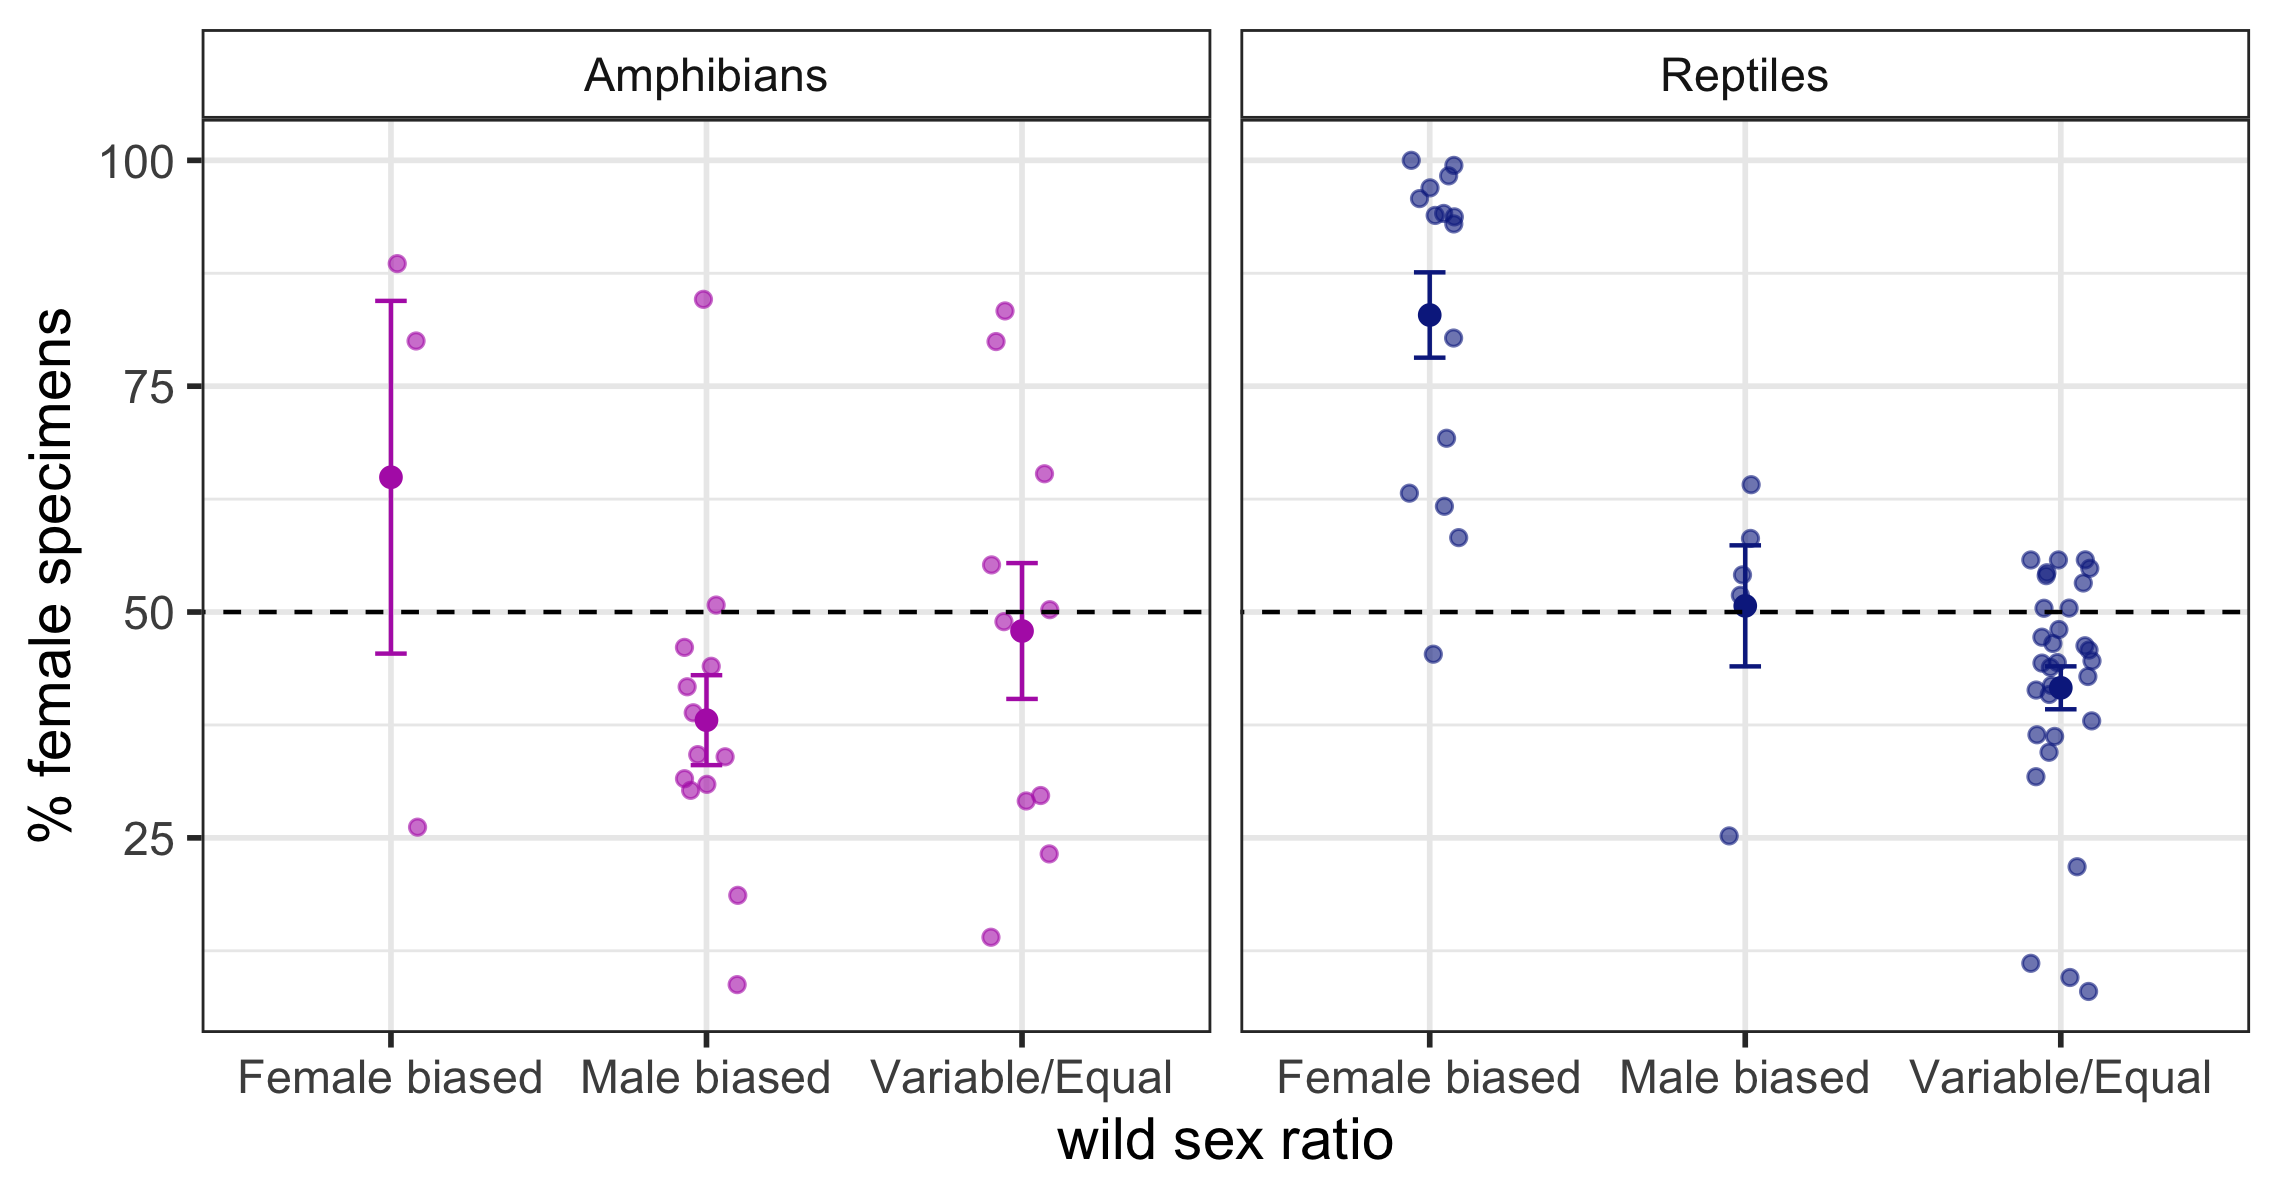
\includegraphics[width = \linewidth]{figures/wild-sex-ratios.png}
%  \caption{Adult sex ratio (ASR) in wild populations versus ASR in our museum dataset for 119 bird species. 
%  Wild ASR values come from Szekely et al. (2014)\cite{szekely2014sex}. 
%  For the museum dataset only species with at least 100 specimens are included. 
%  The dotted lines represents 50\% female specimens in either the wild or museum ASR data. 
%  The red dashed line is the 1:1 line representing where points would sit of wild ASR and museum ASR are identical for a given %species.
%  Points above this line indicate species where museum ASR is more male biased than in wild populations.
%}
%  \label{fig-asr}
%\end{figure}

%-------------------------------------------------------------------------------


%-------------------------------------------------------------------------------
\newpage
% References

% Add reference list for the body size data.


\bibliographystyle{vancouver}
\bibliography{sex-bias}

\end{document}